% A LaTeX template for EXECUTIVE SUMMARY of the MSc Thesis submissions to
% Politecnico di Milano (PoliMi) - School of Industrial and Information Engineering
%
% P. F. Antonietti, S. Bonetti, A. Gruttadauria, G. Mescolini, A. Zingaro
% e-mail: template-tesi-ingind@polimi.it
%
% Last Revision: October 2021
%
% Copyright 2021 Politecnico di Milano, Italy. Inc. All rights reserved.

\documentclass[11pt,a4paper]{article}

%------------------------------------------------------------------------------
%	REQUIRED PACKAGES AND  CONFIGURATIONS
%------------------------------------------------------------------------------
% PACKAGES FOR TITLES
\usepackage{titlesec}
\usepackage{color}

% PACKAGES FOR LANGUAGE AND FONT
\usepackage[utf8]{inputenc}
\usepackage[english]{babel}
\usepackage[T1]{fontenc} % Font encoding
% PACKAGES FOR IMAGES
\usepackage{graphicx}
\graphicspath{{Images/}} % Path for images' folder
\usepackage{eso-pic} % For the background picture on the title page
\usepackage{subfig} % Numbered and caption subfigures using \subfloat
\usepackage{caption} % Coloured captions
\usepackage{transparent}

% STANDARD MATH PACKAGES
\usepackage{amsmath}
\usepackage{amsthm}
\usepackage{bm}
\usepackage[overload]{empheq}  % For braced-style systems of equations

% PACKAGES FOR TABLES
\usepackage{tabularx}
\usepackage{longtable} % tables that can span several pages
\usepackage{colortbl}

% PACKAGES FOR ALGORITHMS (PSEUDO-CODE)
\usepackage{algorithm}
\usepackage{algorithmic}

% PACKAGES FOR REFERENCES & BIBLIOGRAPHY
\usepackage[colorlinks=true,linkcolor=black,anchorcolor=black,citecolor=black,filecolor=black,menucolor=black,runcolor=black,urlcolor=black]{hyperref} % Adds clickable links at references
\usepackage{cleveref}
\usepackage[square, numbers, sort&compress]{natbib} % Square brackets, citing references with numbers, citations sorted by appearance in the text and compressed
\bibliographystyle{plain} % You may use a different style adapted to your field

% PACKAGES FOR THE APPENDIX
\usepackage{appendix}

% PACKAGES FOR ITEMIZE & ENUMERATES
\usepackage{enumitem}

% OTHER PACKAGES
\usepackage{amsthm,thmtools,xcolor} % Coloured "Theorem"
\usepackage{comment} % Comment part of code
\usepackage{fancyhdr} % Fancy headers and footers
\usepackage{lipsum} % Insert dummy text
\usepackage{tcolorbox} % Create coloured boxes (e.g. the one for the key-words)
\usepackage{stfloats} % Correct position of the tables
\usepackage{multirow}
\usepackage{multicol}





%-------------------------------------------------------------------------
%	NEW COMMANDS DEFINED
%-------------------------------------------------------------------------
% EXAMPLES OF NEW COMMANDS -> here you see how to define new commands
\newcommand{\bea}{\begin{eqnarray}} % Shortcut for equation arrays
\newcommand{\eea}{\end{eqnarray}}
\newcommand{\e}[1]{\times 10^{#1}}  % Powers of 10 notation
\newcommand{\mathbbm}[1]{\text{\usefont{U}{bbm}{m}{n}#1}} % From mathbbm.sty
\newcommand{\pdev}[2]{\frac{\partial#1}{\partial#2}}
% NB: you can also override some existing commands with the keyword \renewcommand

%----------------------------------------------------------------------------
%	ADD YOUR PACKAGES (be careful of package interaction)
%----------------------------------------------------------------------------
\usepackage{amsfonts} 
\usepackage[font=footnotesize,labelfont=bf]{caption}

%----------------------------------------------------------------------------
%	ADD YOUR DEFINITIONS AND COMMANDS (be careful of existing commands)
%----------------------------------------------------------------------------
\usepackage{import}
\usepackage{xifthen}
\usepackage{pdfpages}
\usepackage{transparent}
\usepackage{wrapfig}
\usepackage{dsfont}
\usepackage{shadethm}

\parindent=0pt

\newcommand{\incfig}[1]{%
    \def\svgwidth{\columnwidth}
    \import{./Images/}{#1.pdf_tex}
}
\newcommand*{\oldepsilon}{\epsilon}
\renewcommand*{\epsilon}{\varepsilon}
\DeclareMathOperator*{\esssup}{ess\,sup}

\numberwithin{equation}{section}
%----------------------------------------------------------------------------
%	CONFIGURATION OF THEOREM ENVIRONMENTS


% \newtheoremstyle{break}
%     {\partopsep}{\topsep}%  
%     {\normalfont}{}
%     {\bfseries}{}%
%     {\newline}{}%
% \theoremstyle{break}
% \newtheorem{theorem}{Theorem}[section]
% \newtheorem{corollary}{Corollary}[section]
% \newtheorem{proposition}{Proposition}[section]
% \newtheorem{remark}{Remark}[section]
% \newtheorem{lemma}{Lemma}[section]
% \newtheorem{notation}{Notation}[section]
% \newtheorem{definition}{Definition}[section]

% \newtheorem{definition}{Definition}[section]

% \newtheorem*{remark}{Remark}

% \newtheorem{lemma}{Lemma}[section]
% %----------------------------------------------------------------------------

% Do not change Configuration_files/config.tex file unless you really know what you are doing.
% This file ends the configuration procedures (e.g. customizing commands, definition of new commands)
% Set the geometric layout of the document
\usepackage{geometry}
\geometry{
  top=3cm,
  left = 2.0cm,
  right = 2.0cm,
  bottom=2cm,
  headheight= 2cm,
  headsep= 0cm,
}
\raggedbottom

% Create color bluePoli (-> manuale grafica coordinata:  https://www.polimi.it/fileadmin/user_upload/il_Politecnico/grafica-coordinata/2015_05_11_46xy_manuale_grafica_coordinata.pdf)
\definecolor{bluePoli}{cmyk}{0.4,0.1,0,0.4}

% Custom theorem environments
\declaretheoremstyle[
  shaded={rulecolor=bluePoli!20, rulewidth=1pt, bgcolor=bluePoli!5},
  headfont=\color{bluePoli}\normalfont\bfseries,
  bodyfont=\color{black}\normalfont,
]{colored}

\captionsetup[figure]{labelfont={color=bluePoli}} % Set colour of the captions
\captionsetup[table]{labelfont={color=bluePoli}} % Set colour of the captions
\captionsetup[algorithm]{labelfont={color=bluePoli}} % Set colour of the captions

\theoremstyle{colored}
\newtheorem{theorem}{Theorem}[section]
\newtheorem{proposition}{Proposition}[section]
\newtheorem{definition}{Definition}[section]
\newtheorem*{remark}{Remark}
\newtheorem{lemma}{Lemma}[section]

% Enhances the features of the standard "table" and "tabular" environments.
\newcommand\T{\rule{0pt}{2.6ex}}
\newcommand\B{\rule[-1.2ex]{0pt}{0pt}}

% Algorithm description
\newcounter{algsubstate}
\renewcommand{\thealgsubstate}{\alph{algsubstate}}
\newenvironment{algsubstates}{
    \setcounter{algsubstate}{0}%
    \renewcommand{\STATE}{%
    \stepcounter{algsubstate}%
    \Statex {\small\thealgsubstate:}\space}
    }{}

% Custom theorem environment
\newcolumntype{L}[1]{>{\raggedright\let\newline\\\arraybackslash\hspace{0pt}}m{#1}}
\newcolumntype{C}[1]{>{\centering\let\newline\\\arraybackslash\hspace{0pt}}m{#1}}
\newcolumntype{R}[1]{>{\raggedleft\let\newline\\\arraybackslash\hspace{0pt}}m{#1}}

% Custom itemize environment
\setlist[itemize,1]{label=$\bullet$}
\setlist[itemize,2]{label=$\circ$}
\setlist[itemize,3]{label=$-$}
\setlist{nosep}

% Set separation of columns
\setlength{\columnsep}{30pt}

% Create command for background pic
\newcommand\BackgroundPic{% Adding background picture
	\put(230,358){
		\parbox[b][\paperheight]{\paperwidth}{%
			\vfill
			\centering
			\transparent{0.2}
			
\includegraphics[width=0.8\paperwidth]{raggiera_polimi.eps}%
			\vfill
}}}

% Set indentation
%\setlength\parindent{0pt}

% Custom title commands
\titleformat{\section}
{\color{bluePoli}\normalfont\Large\bfseries}
{\color{bluePoli}\thesection.}{1em}{}
\titlespacing*{\section}
{0pt}{2ex}{1ex}

\titleformat{\subsection}
{\color{bluePoli}\normalfont\large\bfseries}
{\color{bluePoli}\thesubsection.}{1em}{}
\titlespacing*{\subsection}
{0pt}{2ex}{1ex}

\titleformat{\subsubsection}
{\color{bluePoli}\normalfont\normalsize\bfseries}
{\color{bluePoli}\thesubsubsection.}{1em}{}
\titlespacing*{\subsubsection}
{0pt}{2ex}{1ex}

% Custom headers and footers
\pagestyle{fancy}
\fancyhf{}

\fancyfoot{}
\fancyfoot[C]{\thepage} % page
\renewcommand{\headrulewidth}{0mm} % headrule width
\renewcommand{\footrulewidth}{0mm} % footrule width

\makeatletter
\patchcmd{\headrule}{\hrule}{\color{black}\hrule}{}{} % headrule
\patchcmd{\footrule}{\hrule}{\color{black}\hrule}{}{} % footrule
\makeatother

% -> Create the header
\chead[C]{
\centering
\begin{tcolorbox}[arc=0pt, boxrule=0pt, colback=bluePoli!60, width=\textwidth, colupper=white]
    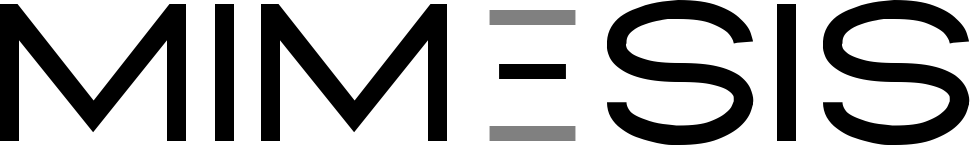
\includegraphics[width=0.2\textwidth]{mimesis.png}
\end{tcolorbox}
}


% Insert here the info that will be displayed into your Title page
% -> title of your work
\renewcommand{\title}{\noindent A Mathematical Model for Alzheimer Disease:

from Microscopic to a Macroscopic Model using
the Two-Scale Homogenization Theory}

% -> author name and surname
\renewcommand{\author}{Andrea Bonifacio}
% -> MSc course
\newcommand\norm[1]{\lVert#1\rVert}
\newcommand{\course}{Methods and Models for Statistical Mechanics}
% -> advisor name and surname
\newcommand{\advisor}{Silvia Lorenzani}
% IF AND ONLY IF you need to modify the co-supervisors you also have to modify the file Configuration_files/title_page.tex (ONLY where it is marked)
%\newcommand{\firstcoadvisor}{Name Surname} % insert if any otherwise comment
%\newcommand{\secondcoadvisor}{Name Surname} % insert if any otherwise comment
% -> academic year
\newcommand{\YEAR}{2023-2024}

%-------------------------------------------------------------------------
%	BEGIN OF YOUR DOCUMENT
%-------------------------------------------------------------------------
\begin{document}
%-----------------------------------------------------------------------------
% TITLE PAGE
%-----------------------------------------------------------------------------
% Do not change Configuration_files/TitlePage.tex (Modify it IF AND ONLY IF you need to add or delete the Co-advisors)
% This file creates the Title Page of the document
% DO NOT REMOVE SPACES BETWEEN LINES!

%\twocolumn[{\begin{@twocolumnfalse}

\AddToShipoutPicture*{\BackgroundPic}

\hspace{-0.6cm}
\includegraphics[width=0.6\textwidth]{logo_polimi_ing_indinf.eps}

\vspace{-1mm}
\fontsize{0.3cm}{0.5cm}\selectfont \bfseries \textsc{\color{bluePoli} Report}\\

\vspace{-0.2cm}
\Large{\textbf{\color{bluePoli}{\title}}}\\

\vspace{-0.2cm}
\fontsize{0.3cm}{0.5cm}\selectfont \bfseries \textsc{\color{bluePoli} \course}\\

\vspace{-0.2cm}
\fontsize{0.3cm}{0.5cm} \selectfont \bfseries Authors: \textsc{\textbf{\author}}\\

%\vspace{-0.4cm}
%\fontsize{0.3cm}{0.5cm}\selectfont \bfseries Advisor: \textsc{\textbf{\advisor}}\\

% if only ONE co-advisor is present:
%\vspace{-0.4cm}
%\fontsize{0.3cm}{0.5cm}\selectfont \bfseries Co-advisor: \textsc{\textbf{\firstcoadvisor}}\\
% if more than one co-advisors are present:
%\vspace{-0.4cm}
%\fontsize{0.3cm}{0.5cm}\selectfont \bfseries Co-advisors: \textsc{\textbf{\firstcoadvisor}}\textsc{\textbf{\secondcoadvisor}}\\

\vspace{-0.4cm}
\fontsize{0.3cm}{0.5cm}\selectfont \bfseries Academic year: \textsc{\textbf{\YEAR}}

\small \normalfont

\vspace{11pt}

\centerline{\rule{1.0\textwidth}{0.4pt}}

%\vspace{15pt}
%\end{@twocolumnfalse}}]

\thispagestyle{plain} % In order to not show the header in the first page


%%%%%%%%%%%%%%%%%%%%%%%%%%%%%%
%%     THESIS MAIN TEXT     %%
%%%%%%%%%%%%%%%%%%%%%%%%%%%%%%
In this work will be presented a mathematical model for Alzheimer's disease (AD) at the microscopic scale. The model will be derived from the Smoluchowski equation, which describes the evolution of the density of diffusing particles that coagulate in pairs. Then will be proved that the model two-scale converges to a macroscopic model asymptotically consistent with the original one. Indeed, the information given on the microscale by the non-homogeneous Neumann boundary condition is transferred into a source term appearing in the limiting (homogenized) equations. Most of this report is based off the work of \cite{Franchi_Lorenzani_2016}, with some additions from \cite{Bertsch}.

%-----------------------------------------------------------------------------
% INTRODUCTION
%-----------------------------------------------------------------------------

\section{Introduction}

Numerical simulations play a critical role in a wide array of scientific and engineering applications, providing insights into the behavior of physical systems under various conditions. Among the most prominent techniques for performing such simulations is Finite Element Modeling (FEM). FEM discretizes a continuous domain into a mesh of finite elements, allowing for the approximation of solutions to complex partial differential equations (PDEs). However, one significant drawback of FEM is its computational intensity, especially when high resolution is required for accurate results. This research aims to explore the potential of Deep Learning (DL) techniques to accelerate FEM simulations, focusing specifically on the deformation of objects subjected to external forces.

The deformation of an object under an applied force is directly tied to the object's discretization. In FEM, the object is represented by a mesh, where the resolution of the mesh—i.e., the size and number of elements—clearly impacts the accuracy and computational cost of the simulation. High-resolution meshes can capture fine details of deformation, leading to more accurate simulations, but they are computationally expensive and time-consuming. 

The main goal of this work is to study the efficacy of a method that combines both Finite Element Modeling (FEM) and DL to obtain a realistic simulation of an object in a fraction of the time that would be required by a traditional FEM simulation. The idea is to, somehow, train a DL model to have inside the information given by the refined discretization and pass them on a coarser discretization.

The idea of using DL techniques to solve scientific problem is not new. Thanks to the rise of new frameworks and libraries, such as TensorFlow and PyTorch, it is now possible to train very complex models on large datasets in a reasonable amount of time. For the problem at hand, a lot of different approaches can be found in the existing literature: a lot of them are based on the idea that the deep learning model should predict the whole dynamic of the system, for example MeshGraphNet \cite{pfaffLearningMeshBasedSimulation2021a} or its multiscale version \cite{fortunatoMultiScaleMeshGraphNets2022}, but these are just two examples of the many possible approaches \cite{jiangMeshfreeFlowNetPhysicsConstrainedDeep2020}, \cite{djeumouNeuralNetworksPhysicsInformed2022}, \cite{hanPredictingPhysicsMeshreduced2022a}. Other methods rely on solving a time independent problem, using various architectures, such as PINNs \cite{djeumouNeuralNetworksPhysicsInformed2022} or GNNs \cite{gaoPhysicsinformedGraphNeural2022}. The proposed method falls into the second category, as it will be explained in the following sections.

One interesting solution is given by \cite{Wang_Du_Coros_Thomaszewski_2024}, where the authors extend the concept of linear modes and modal dynamics \cite{Pentland_Williams_1989} to be able to handle larger deformations. The key idea is to obtain a linear approximation of the deformation, then train a network to minimize the energy of the system, so that for every modal coordinate, the network will learn a non-linear correction, effectively learning a series of non-linear modes. This allows for faster simulations by exploiting subspace dynamics, where the simulation is performed in a reduced space to ease computational costs. The authors show that 


\section{Smoluchowski equation}
The Smoluchowski coagulation equation models various kinds of phenomena as, for example: the evolution of a system of solid or liquid particles suspended in a gas (in
aerosol science), polymerization (in chemistry), aggregation of colloidal particles (in physics), formation of stars and planets (in astrophysics), red blood cell aggregation (in
hematology), behavior of fuel mixtures in engines (in engineering). By convention, only binary reaction will be considered.
This phenomenon is called coalescence and can be written formally as 
\[
    P_i + P_j \rightarrow P_{i+j}
\]
Under the assumption that the aggregation of cluster is the result of only Brownian motion or diffusion, the equations can be written as:
\begin{equation}
    \pdev{u_i}{t}(t,x) - d_i \Delta_x u_i(t,x) = Q_i(u) \quad \text{in } [0,T] \times \Omega,
    \label{eq:smoluchowski}
\end{equation}
where \(u_i\) is the concentration of the cluster of length \(i\), \(d_i\) is the diffusion coefficient, \(\Omega\) is the domain of the system and \(Q_i(u)\) is the gain term minus the loss term which  are defined in this way:
\begin{equation*}
    \begin{aligned}
    &Q_{g, i}=\frac{1}{2} \sum_{j=1}^{i-1} a_{i-j, j} u_{i-j} u_{j} \\
    &Q_{l, i}=u_{i} \sum_{j=1}^{\infty} a_{i, j} u_{j}
    \end{aligned}
\end{equation*}
$Q_{g,i}$ describes the increasing of concentrations of the cluster of length $i$,
$Q_{l,i}$ describes the depletion of the polymers of size $i$.
An important role is played by the coagulation coefficients $a_{i-i,j}$ which describe a situation where a polymer $i-j$ coagulates with a polymer of length $i$ to form one of length $j$, they are symmetric, indeed $a_{i,j}=a_{j,i}$.\\
The \eqref{eq:smoluchowski} is nonlinear and of infinite dimension: the existence and uniqueness of the solution is not guaranteed by the theory of RDEs. The existence of the solution as a matter of facts depends on the choice of the coagulation coefficients, of which an explicit expression is given in \cite{Bertsch}.
If there are no sources the total mass of the clusters will be conserved, but actually this is not true. In fact a particular choice of the coefficients produces a non-conservation of the total mass due to the appearance of an infinite cluster called gel, which is born from the growth of longer and longer clusters (this is known as gelation phenomenon), but will not be discussed here.
\section{The mathematical model for Alzheimer Disease}
As mentioned above, inside the brain there exists a protein called \(\beta\) amyloid peptide ($\mathrm{A} \beta$). Healthy brains produce this protein in monomeric form, but when the mechanism breaks down \(\beta\) starts to auto agglomerate and to form senile plaques. The toxic polymers are the intermediate oligomeric formulation which causes the death of neurons. However, the causes of the AD are not yet completely known, researchers try to study this phenomenon, but the problem is that these intermediate polymers decay very soon in other longer ones. From experiments, it's not easy to study the process of coagulation, therefore the mathematical model helps us to study this process. An assumption that will be made is that 'large' assemblies do not aggregate with each other.
\subsection{Model for the brain}
\begin{figure}[H]
  \centering
  \scalebox{.5}{\incfig{domain_empty}}
  \caption{The domain $\Omega$ representing the cerebral tissue.}
  \label{fig:domain}
\end{figure}
The portion of cerebral tissue considered  in the following is represented by a bounded smooth region $\Omega_{0}\subset \mathbb{R}^3$, whereas the neurons are represented by a family of regular region $\Omega_{j}$ such that:
\begin{enumerate}[label=(\roman*)]
    \item $\bar\Omega_{j}\subset \Omega_{0}$  if   $j=1,2,\dots,\bar{M}$,
    \item $\bar\Omega_{i}\cap \bar\Omega_{j}= \emptyset$  if $i\neq j$.
\end{enumerate}
Let 
$$
\Omega := \Omega_{0} \setminus
\bigcup_{j=1}^{\bar M} \bar\Omega_{j},
$$

\noindent and consider the vector-valued function $u=(u_1,\dots, u_M)$, where $u_j=u_j(t,x)$ $(t\geq 0, t\in \mathbb{R}$ and $x\in \Omega)$ is the molar concentration at the point $x$ and at the time $t$ of a \(\beta\) assembly of $j$ monomers, while $u_M$ takes into account the aggregation of more than $M-1$ monomers. With the definition of $u_M$ it is assumed that `large' assemblies do not aggregate to each other.
Here's a brief presentation of the model made for this problem. Three different stages of the aggregation of \(\beta\) will be considered: its concentration can be modeled with $u_{i}$ with $1\leq i \leq m < M$.
The $u_{1}$ describes the concentration of monomers with the following RDE: 
$$
\frac{\partial u_{1}}{\partial t}(t, x)-d_{1} \Delta_{x} u_{1}(t, x)+u_{1}(t, x) \sum_{j=1}^{M} a_{1, j} u_{j}(t, x)=0.
$$
There is no gain term on the right-hand side because it's impossible for two monomers to coagulate and form another monomer. The loss term is given by the sum of all the possible coagulation of the monomers. 
To solve this equation boundary conditions and initial conditions are necessary.
On the external boundary homogeneous Neumann conditions are assumed, which is meant to artificially isolate the portion of tissue considered from the surrounding environment:
$$
\frac{\partial u_1}{\partial v} \equiv \nabla_{x} u_1\cdot n=0 \quad \text { on }[0, T] \times \partial \Omega.$$
In this way the flux on external fixed boundary is equal to zero, essentially isolating the portion of cerebral tissue from the rest of the world.
Boundary conditions are also needed on the boundaries of the neurons $\partial\Omega_{j}$:
$$ 
\frac{\partial u_{1}}{\partial v} \equiv \nabla_{x} u_1 \cdot n= \psi_{j} \quad \text { on } \partial\Omega_{j}.
$$
This physically models the fact that the neurons produce \(\beta\) in monomeric form. The function $\psi$ is a smooth function and it represents the quantity of \(\beta\) which is produced by the membrane of the neuron, it is a given of the problem.\\
The model considers a portion of the cerebral tissue with a bounded open set $\Omega$ in $\mathbb{R}^{3}$ with a smooth boundary $\partial \Omega$ as seen in Figure \ref{fig:domain}. The neurons in the model will be represented as holes in this domain which are distributed periodically and which have characteristic dimension $0<\epsilon<1$. The set of the domain with the holes is called the perforated domain.
It is assumed that the membrane of the neurons (holes) produces $\mathrm{A} \beta$ and that at time $t=0$ there is no production of  $\mathrm{A} \beta$ from the holes.
Let $Y$ be the unit periodicity cell $\left[0,1\left[{ }^{3}\right.\right.$ having the paving property, shown in Figure \ref{fig:unit_cell}. 
Also, denote by $T$ an open subset of $Y$ with a smooth boundary $\Gamma$, such that $\overline{T} \subset \operatorname{Int} Y$, this means that $T$ can not intersect the boundary of the set $Y$, which is the boundary of the cell. Now call with $Y^{*}=Y \backslash T$ the material part, the "solid part" of the brain. 
\begin{figure}[H]
    \centering
    \scalebox{.5}{\incfig{cell}}
    \caption{The unit periodicity cell $Y$ with the set $T$ of the interior of the hole, bounded by \(\Gamma\)}
    \label{fig:unit_cell}
  \end{figure}

Starting from this it is possible to create a perforated domain: perforate $\Omega$ by removing from it a set $T_{\epsilon}$ of periodically distributed holes defined as before. The set $T$ represents a generic neuron, and $Y^{*}$ the supporting cerebral tissue. Then define $\tau(\epsilon \overline{T})$ to be the set of all translated images $\epsilon \overline{T}$ of the form $\epsilon(k+\overline{T}), k \in \mathbb{Z}^{3}$. Then,

\[ T_{\epsilon} \coloneqq \Omega \cap \tau(\epsilon \overline{T}) . \] is the set of all the holes in the domain.

Introduce now the periodically perforated domain $\Omega_{\epsilon}$ defined by

$$
\Omega_{\epsilon} \coloneqq \Omega \backslash \bar{T}_{\epsilon},
$$
which represent all the set outside the holes. The domain $\Omega_{\epsilon}$ is shown in Figure \ref{fig:perforated_domain}.
\begin{figure}[H]
    \centering
    \scalebox{.5}{\incfig{drawing}}
    \caption{The perforated domain $\Omega_\epsilon$ representing the cerebral tissue. The neurons are represented by the holes.}
    \label{fig:perforated_domain}
  \end{figure}

Ensure that there exists a ``security zone'' where the neurons cannot touch the boundary of \(\Omega\), this is necessary to extend all the functions which live in the solid part also in the holes.
\begin{equation}
  \exists \delta>0 \text { such that dist }\left(\partial\Omega, T_{\epsilon}\right)\geq\delta.
\label{eq:security_zone}
\end{equation}
Therefore can be assumed that $\Omega_{\epsilon}$ is connected. In this scenario there are two boundaries, an internal one $\Gamma_{\epsilon}$, defined by:
$$
\Gamma_{\epsilon} \coloneqq \bigcup\left\{\partial(\epsilon(k+\bar{T})) \mid \epsilon(k+\bar{T}) \subset \Omega\right\}
$$
and an external one that is the fixed exterior boundary denoted by $\partial \Omega$:
$$
\partial\Omega_{\epsilon}\coloneqq\partial\Omega+\Gamma_{\epsilon}.
$$
It is also known that:
\begin{equation}
  \lim _{\epsilon \rightarrow 0} \epsilon\left|\Gamma_{\epsilon}\right|_{N-1}=|\Gamma|_{N-1} \frac{|\Omega|_{N}}{|Y|_{N}}
\label{eq:limit_gamma_eps}
\end{equation}
where $|\cdot|_{N}$ is the $N$-dimensional Hausdorff measure.

The aim is to pass from the microscopic scale to the macroscopic, that is, looking at the brain from 'very high' and we obtain it by performing $\epsilon \rightarrow 0$ which is the scale where clinical data exists. This process is called homogenization theory, and it is a mathematical technique that gives us some mathematical tools to perform this sort of average.
\subsection{The equations}
The system that describes the evolution of monomers is the following:
\begin{equation}
    \begin{dcases}
    \frac{\partial u_{1}^{\epsilon}}{\partial t}(t, x)-d_{1} \Delta_{x} u_{1}^{\epsilon}(t, x)+u_{1}^{\epsilon}(t, x) \sum_{j=1}^{M} a_{1, j} u_{j}^{\epsilon}(t, x)=0, & \text { in }[0, T] \times \Omega_{\epsilon},\\
    \frac{\partial u^{\epsilon}_1}{\partial v} \equiv \nabla_{x} u^{\epsilon}_1\cdot n=0, & \text { on }[0, T]\times\partial\Omega,\\
    \frac{\partial u^{\epsilon}_{1}}{\partial v} \equiv \nabla_{x} u^{\epsilon}_1 \cdot n=\epsilon \psi\left(t, x,\frac{x}{\epsilon}\right), & \text { on }[0, T] \times \Gamma_{\epsilon},\\
    u_{1}^{\epsilon}(0, x)=U_{1}, & \text{ in }\Omega_{\epsilon}.
    \end{dcases}
\label{eq:u_1_eqs}\end{equation}
Note that the $\epsilon$ is put in front of $\psi$ to prevent the divergence of the integral in a further passage, in order to avoid singularities. 
The variable $x$ is called the slow variable and the dependence between $\psi$ and $x$ models the evolution of the disease at a macroscopic scale. The variable
$\frac{x}{\epsilon}$ is called the fast scale variable, which represents the microscopic scale because the main variation of our function are on the scale of the neurons, it's in this small scale that we have a very big change.\\
From our assumptions we suppose that for $t>0$ the brain becomes sick. For technically reasons we have to assume some regularity on $\psi$ and $U_1$:
\begin{enumerate}
    \item $\psi\left(t, x, \frac{x}{\epsilon}\right) \in C^{1}(0, T ; B)$ with $B=C^{1}\left[\bar{\Omega} ; C_{\text {\# }}^{1}(Y)\right]$, where $C_{\#}^{1}(Y)$ is the subset of $C^{1}\left(\mathbb{R}^{N}\right)$ of $Y$-periodic functions;
    \item $\psi\left(t=0, x, \frac{x}{\epsilon}\right)=0$
    \item 
$U_{1}$ is a positive constant such that
\begin{equation}
  U_{1} \leq\|\psi\|_{L^{\infty}(0, T ; B)} .
\label{eq:U_1_norm}\end{equation}
\end{enumerate}
Behind these properties $\psi $ is a generic given function that should be specified in some way if one wants to make the model applicable. We will give an explicit example of it in the last part of the paper.\\
Now we will describe the evolution of oligomers: $1<m<M$. The unknown here is the concentration of a oligomer of generic length $m$
\begin{equation}
    \begin{dcases}
        \frac{\partial u_{m}^{\epsilon}}{\partial t}(t, x)-d_{m} \Delta_{x} u_{m}^{\epsilon}(t, x)+u_{m}^{\epsilon}(t, x) \sum_{j=1}^{M} a_{m, j} u_{j}^{\epsilon}(t, x)= \frac{1}{2} \sum_{j=1}^{m-1} a_{j, m-j} u_{j}^{\epsilon} u_{m-j}^{\epsilon}, & \text { in }[0, T] \times \Omega_{\epsilon},\\
        \frac{\partial u_{m}^{\epsilon}}{\partial v} \equiv \nabla_{x} u_{m}^{\epsilon} \cdot n=0,  & \text { on }[0, T]\times\partial\Omega, \\
        \frac{\partial u_{m}^{\epsilon}}{\partial v} \equiv \nabla_{x} u_{m}^{\epsilon} \cdot n=0, & \text { on }[0, T]\times\Gamma_{\epsilon}.\\ 
     u_{m}^{\epsilon}(0, x)=0 & \text{ in } \Omega_{\epsilon}
    \end{dcases}
\label{eq:u_m_eqs}\end{equation}
In this case we assume homogeneous boundary conditions also on $\Gamma_{\epsilon}$ because we assume that the neurons can't produce \(\beta\) in oligomeric form.
For what it concerns $u_{M}$, it describes the sum of all the densities of all large assemblies of \(\beta\). We are able to do that because in reality when we have a large polymer of \(\beta\) it doesn't  coagulate anymore. 
\begin{equation}
    \begin{dcases}
        \frac{\partial u_{M}^{\epsilon}}{\partial t}(t, x)-d_{M} \Delta_{x} u_{M}^{\epsilon}(t, x)= \frac{1}{2} \sum_{\mathclap{\substack{j+k\geq M\\k,j<M}}} a_{j, k} u_{j}^{\epsilon} u_{k}^{\epsilon}, & \text { in }[0, T] \times \Omega_{\epsilon},\\
        \frac{\partial u_{M}^{\epsilon}}{\partial v} \equiv \nabla_{x} u_{M}^{\epsilon} \cdot n=0,  & \text { on }[0, T]\times\partial\Omega,
        \\
        \frac{\partial u_{M}^{\epsilon}}{\partial v} \equiv \nabla_{x} u_{M}^{\epsilon} \cdot n=0, & \text { on }[0, T]\times\Gamma_{\epsilon},\\ 
        u_{M}^{\epsilon}(0, x)=0, & \text{ in }\Omega_{\epsilon}.
    \end{dcases}
    \label{eq:u_M_eqs}
\end{equation}
In this last system there isn't the loss term because we are assuming that large assemblies do not coagulate with each other.
At this point we want to go from macroscopic to microscopic, trying to compute a sort of average process. Indeed, our aim is to perform the homogenization on the set \eqref{eq:u_1_eqs}-\eqref{eq:u_m_eqs} of equations as $\epsilon \rightarrow 0$, however there is not a clear notion of convergence for the sequence $u_j^{\epsilon}$ $1\geq j \geq M$ which is defined on a varying set $\Omega_{\epsilon}$, which also is random perforated.

\begin{theorem} 
    If $\epsilon>0$, the system \eqref{eq:u_1_eqs}-\eqref{eq:u_m_eqs} has a unique solution
    $$
    \left(u_{1}^{\epsilon}, \ldots, u_{M}^{\epsilon}\right) \in C^{1+\alpha / 2,2+\alpha}\left([0, T] \times \Omega_{\epsilon}\right) \quad(\alpha \in(0,1))
    $$
    such that
    $$
    u_{j}^{\epsilon}(t, x)>0 \text { for }(t, x) \in(0, T) \times \Omega_{\epsilon}, j=1, \ldots, M .
    $$
    \label{thm:3.1}
\end{theorem}

\section{Two-Scale Convergence}

\begin{definition}[Two-scale convergence]
A sequence of functions $ v ^ {\epsilon } $in $ L^2([ 0 ,T]\times\Omega) $ two-scale converges to $v_{0} \in L^2([ 0 ,T]\times\Omega \times Y)$ if
$$
\lim_{\epsilon \to 0} \int_{0}^{\textrm{T}} \int_{\Omega} v^{\epsilon}(t,x)\psi\left(t,x,\frac{x}{\epsilon}\right) \, dxdt=\int_{0}^{\textrm{T}} \int_{\Omega} \int_{\textrm{Y}} v(t,x,y)\psi(t,x,y) \, dydxdt
$$ 
for all $\psi \in C^1([0,T]\times \bar\Omega;C_{\#}^{\infty}(Y))$
\label{def 7.1}\end{definition}
This definition makes sense because of the next compactness theorem 
\begin{theorem}[Compactness Theorem]
If $v^{\epsilon}$ is a bounded sequence in $ L^2([ 0 ,T]\times\Omega) $, then there exist a function $v_{0}(t,x,y) \in   L^2([0,T]\times\Omega \times Y)$ s.t. $v^{\epsilon}$ two-scale converges to $v_{0}$, we write: 
$v^{\epsilon} \overset{2s}{\rightharpoonup} v_{0}$.
\label{thm 7.1}\end{theorem}
This theorem is important because it shows that the minimal requirement to have two-scale convergence is that $v$ must be bounded. Notice that the two-scale limit contains one more variable with respect to the first one, that is the $y$ variable. It represent the small scale and it reflects the fluctuations of our model on the microscale.
\begin{remark}[Remark, relation with weak convergence] If we assume that $\psi$ is independent of $y$, and ignoring the dependence on time (since the homogenization is performed on the spatial grid) we obtain:
$$ 
\lim_{\epsilon \to 0} \int_{\Omega} v^{\epsilon}(x)\psi(x)dx= \int_{\Omega} \int_{\textrm{Y}} v(x,y)\psi(x)dxdy=\int_{\Omega} \left[\int_{\textrm{Y}} v(x,y)dy\right]\psi(x)dx
$$This shows that, in this specific case, the two-scale convergence coincides with the weak convergence.
In this definition the time is only a parameter, and if we assume that $\psi$ does not depend on $y$ we obtain the definition of weak limit. So in this case the weak limit coincides with the two-scale limit. Therefore the two-scale convergence and the weak convergence are strictly related: the main difference between them is that in the first one the oscillations are captured due to the extra variable $y$.
\end{remark}

\section{Homogenization of the Smoluchowsky equation}
The idea is to try to homogenize the problem, conveniently reported again here:
\begin{equation}
    \begin{dcases}\frac{\partial u_{1}^{\epsilon}}{\partial t}-\operatorname{div}\left(d_{1} \nabla_{x} u_{1}^{\epsilon}\right)+u_{1}^{\epsilon} \sum_{j=1}^{M} a_{1, j} u_{1}^{\epsilon}=0, & \text { in }[0, T] \times \Omega_{\epsilon}, \\ 
    \frac{\partial u_{1}^{\epsilon}}{\partial v} \equiv \nabla_{x} u_{1}^{\epsilon} \cdot n=0, & \text { on }[0, T]\times\partial\Omega,\\ 
    \frac{\partial u_{1}^{\epsilon}}{\partial \nu} \equiv \nabla_{x} u_{1}^{\epsilon} \cdot n=\epsilon \psi\left(t, x, \frac{x}{\epsilon}\right), & \text { on }[0, T] \times \Gamma_{\epsilon} \\ u_{1}^{\epsilon}(0, x)=U_{1}, & \text { in } \Omega_{\epsilon}.
    \end{dcases}
\label{eq 10}\end{equation}
now letting $\epsilon \rightarrow 0$ we pass on a description on the large scale, but to do this, due to previous definitions we need to prove the boundedness of $u_{j}^{\epsilon}, \nabla u_{j}^{\epsilon}, \partial_{t} u_{j}^{\epsilon}$.

\subsection{Preliminary a Priori Estimates}

Since the homogenization will be carried out in the framework of two-scale convergence, the first necessary step is to obtain the a priori estimates for the sequences $u_{j}^{\epsilon}, \nabla u_{j}^{\epsilon}, \partial_{t} u_{j}^{\epsilon}$ in $[0, T] \times \Omega_{\epsilon}$.
Since
$$
\operatorname{div}\left(d_{1} \nabla_{x} u_{1}^{\epsilon}\right)-\frac{\partial u_{1}^{\epsilon}}{\partial t} \geq 0
$$
by the classical maximum principle \cite{Protter_Weinberger_1984}, the following estimate holds.
\begin{lemma} Let $T>0$ be arbitrary and $u_{1}^{\epsilon}$ be a classical solution of \eqref{eq 10}. Then,
\begin{equation} \left\|u_{1}^{\epsilon}\right\|_{L^{\infty}\left(0, T ; L^{\infty}\left(\Omega_{\epsilon}\right)\right)} \leq\left|U_{1}\right|+\left\|u_{1}^{\epsilon}\right\|_{L^{\infty}\left(0, T ; L^{\infty}\left(\Gamma_{\epsilon}\right)\right)}. 
\label{eq 20}\end{equation}
\label{lemma 5.1}\end{lemma}
\begin{lemma} Let $T>0$ be arbitrary and $u_{1}^{\epsilon}$ be a classical solution of \eqref{eq 10}. Then,
\begin{equation}
    \left\|u_{1}^{\epsilon}\right\|_{L^{\infty}\left(0, T ; L^{\infty}\left(\Gamma_{\epsilon}\right)\right)} \leq c\|\psi\|_{L^{\infty}(0, T ; B)},
\label{eq 21}\end{equation}where $c$ is independent of $\epsilon$.
\label{lemma 5.2}\end{lemma}
Thus, the boundedness of $u_{1}^{\epsilon}(t, x)$ in $L^{\infty}\left([0, T] \times \Gamma_{\epsilon}\right)$, uniformly in $\epsilon$, can be immediately deduced from Lemma \eqref{lemma 5.2} applying Lemma \eqref{lemma 5.1}.
In order to establish Lemma \eqref{lemma 5.2}, it will be necessary the following preliminary results, Theorem \eqref{theorem 5.2} and Lemma \eqref{lemma 5.3}.
The following is Lemma 5.6 from \cite{Ladyzenskaja_Solonnikov_Uralceva_1968}.
\begin{lemma}Let $\left(\tilde{z}_{n}\right)_{n \in \mathbb{N}_{0}}$ be a sequence of nonnegative real numbers such that
\begin{equation}
    \tilde{z}_{n+1} \leq c b^{n} \tilde{z}_{n}^{r / 2}   
    \label{eq 22}
\end{equation}
for all $n \in \mathbb{N}_{0}$, with fixed positive constants $c, b, r$, where $b>1$ and
$$
    r=\frac{2(N+1)}{N}>2 .
$$
If
\begin{equation}
    \tilde{z}_{0} \leq \theta\coloneqq c^{-N} b^{-N^{2}}
\label{eq 23}
\end{equation}
then,
\begin{equation}
    \tilde{z}_{n} \leq \theta b^{-n N}
\label{eq 24}
\end{equation}
for all $n \in \mathbb{N}_{0}$.
\label{lemma 5.3}
\end{lemma}
\begin{theorem} Assume that there exist positive constants $T, \hat{k}=\|\psi\|_{L^{\infty}(0, T ; B)}, \gamma$, such that for all $k \geq \hat{k}$ we have
\begin{equation}
    \left\|u_{\epsilon}^{(k)}\right\|_{Q_{\epsilon}(T)}^{2}\coloneqq \sup _{0 \leq t \leq T} \int_{\Omega_{\epsilon}}\left|u_{\epsilon}^{(k)}\right|^{2} \, dx+\int_{0}^{T} \, dt \int_{\Omega_{\epsilon}}\left|\nabla u_{\epsilon}^{(k)}\right|^{2} \, dx \leq \epsilon \gamma k^{2} \int_{0}^{T} \, dt\left|B_{k}^{\epsilon}(t)\right|,
\label{eq 25}\end{equation}
where $u_{\epsilon}^{(k)}(t)\coloneqq \left(u_{1}^{\epsilon}(t)-k\right)_{+}$ and $B_{k}^{\epsilon}(t)$ is the set of points on $\Gamma_{\epsilon}$ at which $u_{1}^{\epsilon}(t, x)>k$.
Then
\begin{equation}
    \operatorname{\esssup }_{(t, x) \in[0, T] \times \Gamma_{\epsilon}} u_{1}^{\epsilon}(t, x) \leq 2 m \hat{k},
\label{eq 26}
\end{equation}
where the positive constant $m$ is independent of $\epsilon$.
\label{theorem 5.2}
\end{theorem}
\begin{proof} Choose
$$
    r=\frac{2(N+1)}{N}>2
$$
Then, it holds
\begin{equation}
    \frac{1}{r}+\frac{(N-1)}{2 r}=\frac{N}{2N+2}+\frac{(N-1)N}{4N+4}=\frac{N}{4}.
\label{eq 27}
\end{equation}
Let $\mathcal{M} \geq \hat{k}$ be arbitrary and define


\begin{align}
    k_{n} &\coloneqq \left(2-2^{-n}\right) \mathcal{M} \geq \hat{k},  \nonumber \\
    z_{n} &\coloneqq \epsilon^{2 / r}\left[\int_{0}^{T} \, d  t\left|B_{k_{n}}^{\epsilon}(t)\right|\right]^{2 / r}
\label{eq 28}
\end{align}
for all $n \in \mathbb{N}_{0}$. To prove now that the sequence $\left(z_{n}\right)$ satisfies the assumptions of \eqref{lemma 5.3}, let $n \in \mathbb{N}_{0}$ be fixed. From the trivial estimate
\begin{equation}
 \left|u_{\epsilon}^{\left(k_{n}\right)}(t)\right|^{2} \geq\left(k_{n+1}-k_{n}\right)^{2} \mathds{1}_{B_{k_{n+1}}^{\epsilon}}{ }^{(t)}
\label{eq 29}\end{equation}
is obtained
\begin{equation}
    \begin{aligned}
        z_{n+1} & \leq \epsilon^{2 / r}\left[\int_{0}^{T} \, d  t\left(k_{n+1}-k_{n}\right)^{-r} \int_{\Gamma_{\epsilon}}\left|u_{\epsilon}^{\left(k_{n}\right)}(t)\right|^{r} \, d  \sigma_{\epsilon}(x)\right]^{2 / r} \\
        &=\left(k_{n+1}-k_{n}\right)^{-2} \epsilon^{2 / r}\left[\int_{0}^{T} \, d  t \int_{\Gamma_{\epsilon}}\left|u_{\epsilon}^{\left(k_{n}\right)}(t)\right|^{r} \, d  \sigma_{\epsilon}(x)\right]^{2 / r}.
    \end{aligned}
\label{eq 30}
\end{equation}
Hence, since the condition \eqref{eq 27} holds, by using \eqref{eq 120}, is obtained
\begin{equation}
    \begin{aligned}
        &2^{-2(n+1)} \mathcal{M}^{2} z_{n+1}=\left(k_{n+1}-k_{n}\right)^{2} z_{n+1} \\
        &\leq c \epsilon^{2 / r} \epsilon^{-N-\left[\frac{2(1-N)}{r}\right]}\left\|u_{\epsilon}^{\left(k_{n}\right)}\right\|_{Q_{\epsilon}(T)}^{2},
    \end{aligned}
\label{eq 31}
\end{equation}
where $c$ is a positive constant independent of $\epsilon$. Therefore,
\begin{equation}
    2^{-2(n+1)} \mathcal{M}^{2} z_{n+1} \leq c \epsilon^{-\frac{N}{(1+N)}}\left\|u_{\epsilon}^{\left(k_{n}\right)}\right\|_{Q_{\epsilon}(T)}^{2}
\label{eq 32}
\end{equation}
Moreover, from \eqref{eq 25} and \eqref{eq 28}:
\begin{equation}
    \begin{aligned}
        \left\|u_{\epsilon}^{\left(k_{n}\right)}\right\|_{Q_{\epsilon}(T)}^{2} & \leq \gamma k_{n}^{2} z_{n}^{r / 2} \leq \gamma\left(2-2^{-n}\right)^{2} \mathcal{M}^{2} z_{n}^{r / 2} \\
        & \leq 4 \gamma \mathcal{M}^{2} z_{n}^{r / 2}.
    \end{aligned}
\label{eq 33}\end{equation}
Combining \eqref{eq 32} and \eqref{eq 33}, is obtained
\begin{equation}
    z_{n+1} \leq c_{0} \epsilon^{-\frac{N}{(1+N)}} 2^{2 n} z_{n}^{r / 2},
\label{eq 34}
\end{equation}
where $c_{0}$ is a positive constant independent of $\epsilon$.
Define
$$
    \begin{aligned}
        &d\coloneqq \frac{(r-2)}{r}, \\
        &\lambda\coloneqq \left(c_{0}\right)^{-\frac{r}{(r-2)}} 2^{-\frac{4}{(r-2) d}},
    \end{aligned}
$$
and choose
\begin{equation}
  \mathcal{M}\coloneqq \hat{k}+\lambda^{-1 / r} \sqrt{c^{\prime}} \hat{k} \equiv m \hat{k},
\label{eq 35}\end{equation}
where $c^{\prime}$ is defined in \eqref{eq 36} and $m>1$. Now should be optimal to estimate $z_{0}$ for the fixed value of $\mathcal{M}$ given by \eqref{eq 35}. From the definition \eqref{eq 28} and \eqref{eq:limit_gamma_eps}, by following the same strategy which leads to \eqref{eq 32} and \eqref{eq 33}, where $\hat{k}$ is substituted for $k_{n}$ and $\mathcal{M}$ for $k_{n+1}$, have that
\begin{equation}
    \begin{aligned}
        (\mathcal{M}-\hat{k})^{2} z_{0} \leq c \epsilon^{-\frac{N}{(1+N)}}\left\|u_{\epsilon}^{(\hat{k})}\right\|_{Q_{\epsilon}(T)}^{2} & \leq c \epsilon^{-\frac{N}{(1+N)}}\left[\gamma \hat{k}^{2} T \frac{|\Gamma|_{N-1}|\Omega|_{N}}{|Y|_{N}}\right] \\
        &\coloneqq c^{\prime} \epsilon^{-\frac{N}{(1+N)} \hat{k}^{2}},
    \end{aligned}
\label{eq 36}
\end{equation}
so that
\begin{equation}
    z_{0} \leq \frac{c^{\prime} \epsilon^{-\frac{N}{(1+N)}} \hat{k}^{2}}{(\mathcal{M}-\hat{k})^{2}}
\label{eq 37}
\end{equation}
for all $\mathcal{M} \geq \hat{k}$. Therefore, from \eqref{eq 37} and \eqref{eq 35}, obtain that
\begin{equation}
    z_{0} \leq \epsilon^{-\frac{N}{(1+N)}} \lambda^{2 / r}.
\label{eq 38}
\end{equation}
For a fixed $\epsilon$, set
\begin{equation}
    \tilde{z}_{n}=\epsilon^{\frac{N}{(1+N)}} z_{n}
\label{eq 39}
\end{equation}
for all $n \in \mathbb{N}_{0}$. Then, the recursion inequality \eqref{eq 34} and the estimate \eqref{eq 38} can be rewritten as follows:
\begin{equation}
    \begin{cases}
        \tilde{z}_{n+1} \leq c_{0} 2^{2 n} \epsilon^{-1} \tilde{z}_{n}^{r / 2}, \\
        \tilde{z}_{0} \leq \lambda^{2 / r}=\left(c_{0}\right)^{-N} 2^{-2 N^{2}}.
    \end{cases}
\label{eq 40}
\end{equation}
Keeping in mind \eqref{eq 40}, it is easy to see that the sequence $\left(\tilde{z}_{n}\right)$ satisfies the assumptions of Lemma \eqref{lemma 5.3} with
$$
    c\coloneqq \max \left\{c_{0}, \frac{c_{0}}{\epsilon}\right\} \text { and } b\coloneqq 4.
$$
Therefore, in view of Lemma \eqref{lemma 5.3}, one can conclude that $z_{n} \rightarrow 0$ as $n \rightarrow \infty$, which implies
$$
    u_{1}^{\epsilon} \leq \lim _{n \rightarrow \infty} k_{n}=2 \mathcal{M}
$$
a.e. on $\Gamma_{\epsilon}$ for almost every $t \in[0, T]$ if we define $\mathcal{M}$ as in \eqref{eq 35}. This gives \eqref{eq 26}.
\end{proof}
Now it is possible to prove Lemma \eqref{lemma 5.2}
\begin{proof} Let $T>0$ and $k \geq 0$ be fixed. Define: $u_{\epsilon}^{(k)}(t)\coloneqq \left(u_{1}^{\epsilon}(t)-k\right)_{+}$ for $t \geq 0$, with derivatives:
\begin{equation}
    \frac{\partial u_{\epsilon}^{(k)}}{\partial t} =\frac{\partial u_{1}^{\epsilon}}{\partial t} \mathbbm{1}_{\left\{u_{1}^{\epsilon}>k\right\}},
\label{eq 41}
\end{equation}
\begin{equation}
    \nabla_{x} u_{\epsilon}^{(k)} =\nabla_{x} u_{1}^{\epsilon} \mathbbm{1}_{\left\{u_{1}^{\epsilon}>k\right\}} .
\label{eq 42}
\end{equation}
Moreover,
\begin{equation}
    \left.u_{\epsilon}^{(k)}\right|_{\partial \Omega}=\left(\left.u_{1}^{\epsilon}\right|_{\partial \Omega}-k\right)_{+},
\label{eq 43}
\end{equation}
\begin{equation}
    \left.u_{\epsilon}^{(k)}\right|_{\Gamma_{\epsilon}}=\left(\left.u_{1}^{\epsilon}\right|_{\Gamma_{\epsilon}}-k\right)_{+}.
\label{eq 44}
\end{equation}
Assume $k \geq \hat{k}$, where $\hat{k}\coloneqq \|\psi\|_{L^{\infty}(0, T ; B)}$. Then, recalling that $U_{1} \leq\|\psi\|_{L^{\infty}(0, T ; B)}$,
\begin{equation}
    u_{1}^{\epsilon}(0, x)=U_{1} \leq \hat{k} \leq k
\label{eq 45}
\end{equation}
For $t \in\left[0, T_{1}\right]$ with $T_{1} \leq T$, obtain (recall that \(\frac{\mathrm{d}}{\mathrm{d} s}\frac{1}{2} \left|u_{\epsilon}^{(k)}(s)\right|^{2} = \frac{\partial u_{\epsilon}^{(k)}(s)}{\partial s} u_{\epsilon}^{(k)}(s)\)):
\begin{equation}
    \begin{aligned}
        \frac{1}{2} \int_{\Omega_{\epsilon}}\left|u_{\epsilon}^{(k)}(t)\right|^{2} \, d  x &=\int_{0}^{t} \frac{d}{ds}\left[\frac{1}{2} \int_{\Omega_{\epsilon}}\left|u_{\epsilon}^{(k)}(s)\right|^{2} \,d x\right] \, ds = \\
        &=\int_{0}^{t} \, ds \int_{\Omega_{\epsilon}} \frac{\partial u_{\epsilon}^{(k)}(s)}{\partial s} u_{\epsilon}^{(k)}(s) \, dx
    \end{aligned} 
\label{eq 46}\end{equation}
Taking into account \eqref{eq 41}, \eqref{eq 10} and Lemma \eqref{lemma 7.1}, it is possible to obtain that for all $s \in\left[0, T_{1}\right]$
\begin{equation}
  \begin{aligned}
        &\int_{\Omega_{\epsilon}} \frac{\partial u_{\epsilon}^{(k)}(s)}{\partial s} u_{\epsilon}^{(k)}(s) \, dx \underset{\eqref{eq 41}}{=}\int_{\Omega_{\epsilon}} \frac{\partial u_{1}^{\epsilon}(s)}{\partial s} u_{\epsilon}^{(k)}(s) \, dx \\
        &\underset{\eqref{eq 10}}{=}\int_{\Omega_{\epsilon}}\left[d_{1} \Delta_{x} u_{1}^{\epsilon}-u_{1}^{\epsilon} \sum_{j=1}^{M} a_{1, j} u_{j}^{\epsilon}\right] u_{\epsilon}^{(k)}(s) \, dx \\
        &\underset{\mathclap{\text{\tiny div. thm}}}{=}-\int_{\Omega_{\epsilon}} u_{1}^{\epsilon}(s) \sum_{j=1}^{M} a_{1, j} u_{j}^{\epsilon}(s) u_{\epsilon}^{(k)}(s) \, dx+d_{1} \int_{\Gamma_{\epsilon}} \nabla_{x} u^{\epsilon}_1 \cdot n u_{\epsilon}^{(k)}(s) \, {d} \sigma_{\epsilon}(x)-d_{1} \int_{\Omega_{\epsilon}} \nabla_{x} u_{1}^{\epsilon}(s) \cdot \nabla_{x} u_{\epsilon}^{(k)}(s) \, dx \\
        &\underset{\eqref{eq 10}}{=}-\int_{\Omega_{\epsilon}} u_{1}^{\epsilon}(s) \sum_{j=1}^{M} a_{1, j} u_{j}^{\epsilon}(s) u_{\epsilon}^{(k)}(s) {d} x+\epsilon d_{1} \int_{\Gamma_{\epsilon}} \psi\left(s, x, \frac{x}{\epsilon}\right) u_{\epsilon}^{(k)}(s) \, {d}\sigma_{\epsilon}(x)
        -d_{1} \int_{\Omega_{\epsilon}} \nabla_{x} u_{1}^{\epsilon}(s) \cdot \nabla_{x} u_{\epsilon}^{(k)}(s) \, {d} x \\
        &\leq \epsilon d_{1} \int_{\Gamma_{\epsilon}} \psi\left(s, x, \frac{x}{\epsilon}\right) u_{\epsilon}^{(k)}(s) \, {d} \sigma_{\epsilon}(x)-d_{1} \int_{\Omega_{\epsilon}} \nabla_{x} u_{1}^{\epsilon}(s) \cdot \nabla_{x} u_{\epsilon}^{(k)}(s) \, {d} x \\
        &\underset{\substack{\text{Young ineq.}\\\text{and}\\\text{def. of } B_{k}^{\epsilon}(t)}}{\leq} \frac{\epsilon d_{1}}{2} \int_{B_{k}^{\epsilon}(s)}\left|\psi\left(s, x, \frac{x}{\epsilon}\right)\right|^{2} \, {d} \sigma_{\epsilon}(x)+\frac{\epsilon d_{1}}{2} \int_{\Gamma_{\epsilon}}\left|u_{\epsilon}^{(k)}(s)\right|^{2} \, {d} \sigma_{\epsilon}(x) -d_{1} \int_{\Omega_{\epsilon}} \nabla_{x} u_{1}^{\epsilon}(s) \cdot \nabla_{x} u_{\epsilon}^{(k)}(s) \, {d} x \\
        &\underset{\eqref{lemma 7.1}}{\leq} \frac{\epsilon d_{1}}{2} \int_{B_{k}^{\epsilon}(s)}\left|\psi\left(s, x, \frac{x}{\epsilon}\right)\right|^{2} \, {d} \sigma_{\epsilon}(x)+\frac{C_{1} d_{1}}{2} \int_{A_{k}^{\epsilon}(s)}\left|u_{\epsilon}^{(k)}(s)\right|^{2} \, {d} x -d_{1}\left(1-\frac{C_{1} \epsilon^{2}}{2}\right) \int_{\Omega_{\epsilon}}\left|\nabla_{x} u_{\epsilon}^{(k)}(s)\right|^{2} \, {d} x,
   \end{aligned}
\label{eq 47}\end{equation}
where is denoted by $A_{k}^{\epsilon}(t)$ and $B_{k}^{\epsilon}(t)$ the set of points in $\Omega_{\epsilon}$ and on $\Gamma_{\epsilon}$, respectively, at which $u_{1}^{\epsilon}(t, x)>k$. It holds:
$$
\begin{aligned}
&\left|A_{k}^{\epsilon}(t)\right| \leq\left|\Omega_{\epsilon}\right|, \\
&\left|B_{k}^{\epsilon}(t)\right| \leq\left|\Gamma_{\epsilon}\right|,
\end{aligned}
$$
with $|\cdot|$ being the natural Hausdorff measure.
Plugging \eqref{eq 47} into \eqref{eq 46} and varying over $t$, it is possible to arrive at the estimate: 
\begin{equation}
  \begin{aligned}
&\sup _{0 \leq t \leq T_{1}}\left[\frac{1}{2} \int_{\Omega_{\epsilon}}\left|u_{\epsilon}^{(k)}(t)\right|^{2} \, d  x\right]+d_{1}\left(1-\frac{C_{1} \epsilon^{2}}{2}\right) \int_{0}^{T_{1}} \, d  t \int_{\Omega_{\epsilon}}\left|\nabla u_{\epsilon}^{(k)}(t)\right|^{2} \, d  x \\
&\leq \frac{C_{1} d_{1}}{2} \int_{0}^{T_{1}} \, d  t \int_{A_{k}^{\epsilon}(t)}\left|u_{\epsilon}^{(k)}(t)\right|^{2} \, d  x+\frac{\epsilon d_{1}}{2} \int_{0}^{T_{1}} \, d  t \int_{B_{k}^{\epsilon}(t)}\left|\psi\left(t, x, \frac{x}{\epsilon}\right)\right|^{2} \, d  \sigma_{\epsilon}(x).
\end{aligned}
\label{eq 48}\end{equation}
Introducing the following norm
\begin{equation}
  \|u\|_{Q_{\epsilon}(T)}^{2}\coloneqq \sup _{0 \leq t \leq T} \int_{\Omega_{\epsilon}}|u(t)|^{2} \, d  x+\int_{0}^{T} \, d  t \int_{\Omega_{\epsilon}}|\nabla u(t)|^{2} \, d  x,
\label{eq 49}\end{equation}
the inequality \eqref{eq 48} can be rewritten as follows:
\begin{equation}
  \begin{aligned}
\min \left\{\frac{1}{2}, d_{1}\left(1-\frac{C_{1} \epsilon^{2}}{2}\right)\right\}\left\|u_{\epsilon}^{(k)}\right\|_{Q_{\epsilon}\left(T_{1}\right)}^{2} \leq & \frac{C_{1} d_{1}}{2} \int_{0}^{T_{1}} \, d  t \int_{A_{k}^{\epsilon}(t)}\left|u_{\epsilon}^{(k)}(t)\right|^{2} \, d  x \\
&+\frac{\epsilon d_{1}}{2} \int_{0}^{T_{1}} \, d  t \int_{B_{k}^{\epsilon}(t)}\left|\psi\left(t, x, \frac{x}{\epsilon}\right)\right|^{2} \, d  \sigma_{\epsilon}(x).
\end{aligned}
\label{eq 50}\end{equation}
It is possible to estimate the right-hand side of \eqref{eq 50}. From Hölder's inequality, obtain
\begin{equation}
  \int_{0}^{T_{1}} \, d  t \int_{A_{k}^{\epsilon}(t)}\left|u_{\epsilon}^{(k)}(t)\right|^{2} \, d  x \leq\left\|u_{\epsilon}^{(k)}\right\|_{L^{\bar{r}_{1}}\left(0, T_{1} ; L^{\bar{q}_{1}}\left(\Omega_{\epsilon}\right)\right)}^{2}\left\|\mathbbm{1}_{A_{k}^{\epsilon}}\right\|_{L^{r_{1}^{\prime}}\left(0, T_{1} ; L^{q_{1}^{\prime}}\left(\Omega_{\epsilon}\right)\right)},
\label{eq 51}\end{equation}
with $r_{1}^{\prime}=\frac{r_{1}}{r_{1}-1}, q_{1}^{\prime}=\frac{q_{1}}{q_{1}-1}, \bar{r}_{1}=2 r_{1}, \bar{q}_{1}=2 q_{1}$, where, for $N>2, \bar{r}_{1} \in(2, \infty)$ and $\bar{q}_{1} \in\left(2, \frac{2 N}{(N-2)}\right)$ have been chosen such that
$$
\frac{1}{\bar{r}_{1}}+\frac{N}{2 \bar{q}_{1}}=\frac{N}{4}.
$$
In particular, $r_{1}^{\prime}, q_{1}^{\prime}<\infty$, so that \eqref{eq 51} yields
\begin{equation}
  \int_{0}^{T_{1}} \, d  t \int_{A_{k}^{\epsilon}(t)}\left|u_{\epsilon}^{(k)}(t)\right|^{2} \, d  x \leq\left\|u_{\epsilon}^{(k)}\right\|_{L^{\overline{r_{1}}\left(0, T_{1} ; L^{\bar{q}_{1}}\left(\Omega_{\epsilon}\right)\right)}}^{2}|\Omega|^{1 / q_{1}^{\prime}} T_{1}^{1 / r_{1}^{\prime}} .
\label{eq 52}\end{equation}
If one chooses
$$
T_{1}^{1 / r_{1}^{\prime}}<\frac{\min \left\{1, d_{1}\right\}}{2 C_{1} d_{1}}|\Omega|^{-1 / q_{1}^{\prime}} \leq \frac{\min \left\{\frac{1}{2}, d_{1}\left(1-\frac{C_{1} \epsilon^{2}}{2}\right)\right\}}{C_{1} d_{1}}|\Omega|^{-1 / q_{1}^{\prime}},
$$
then from \eqref{eq 117}, it follows that
\begin{equation}
  \frac{C_{1} d_{1}}{2} \int_{0}^{T_{1}} \, d  t \int_{A_{k}^{\epsilon}(t)}\left|u_{\epsilon}^{(k)}(t)\right|^{2} \, d  x \leq \frac{1}{2} \min \left\{\frac{1}{2}, d_{1}\left(1-\frac{C_{1} \epsilon^{2}}{2}\right)\right\}\left\|u_{\epsilon}^{(k)}\right\|_{Q_{\epsilon}\left(T_{1}\right)}^{2}.
\label{eq 53}\end{equation}
Analogously, from Hölder's inequality, it is possible to have, for $k \geq \hat{k}$
\begin{equation}
  \begin{aligned}
\frac{\epsilon d_{1}}{2} \int_{0}^{T_{1}} \, d  t \int_{B_{k}^{\epsilon}(t)}\left|\psi\left(t, x, \frac{x}{\epsilon}\right)\right|^{2} \, d  \sigma_{\epsilon}(x) & \leq \frac{\epsilon d_{1} k^{2}}{2}\left(\frac{\hat{k}^{2}}{k^{2}}\right)\left\|\mathds{1}_{B_{k}^{\epsilon}}\right\|_{L^{1}\left(0, T_{1} ; L^{1}\left(\Gamma_{\epsilon}\right)\right)} \\
& \leq \frac{\epsilon d_{1} k^{2}}{2} \int_{0}^{T_{1}} \, d  t\left|B_{k}^{\epsilon}(t)\right| .
\end{aligned}
\label{eq 54}\end{equation}
Thus \eqref{eq 50} yields
\begin{equation}
  \left\|u_{\epsilon}^{(k)}\right\|_{Q_{\epsilon}\left(T_{1}\right)}^{2} \leq \epsilon \gamma k^{2} \int_{0}^{T_{1}} \, d  t\left|B_{k}^{\epsilon}(t)\right| .
\label{eq 55}\end{equation}
Hence, by Theorem \eqref{theorem 5.2}, one obtains
$$
\left\|u_{1}^{\epsilon}\right\|_{L^{\infty}\left(0, T_{1} ; L^{\infty}\left(\Gamma_{\epsilon}\right)\right)} \leq 2 m \hat{k}
$$
where the positive constant $m$ is independent of $\epsilon$. Analogous arguments are valid for the cylinder $\left[T_{s}, T_{s+1}\right] \times \Omega_{\epsilon}, s=1,2, \ldots, p-1$ with
$$
\left[T_{s+1}-T_{s}\right]^{1 / r_{1}^{\prime}}<\frac{\min \left\{1, d_{1}\right\}}{2 C_{1} d_{1}}|\Omega|^{-1 / q_{1}^{\prime}}
$$
and $T_{p} \equiv T$. Thus, after a finite number of steps, it is possible to obtain the estimate \eqref{eq 21}.
\end{proof}
\begin{lemma}
  The sequence $\nabla_{x} u_{1}^{\epsilon}$ is bounded in $L^{2}\left([0, T] \times \Omega_{\epsilon}\right)$, uniformly in $\epsilon$.
\label{lemma 5.4}\end{lemma}
\begin{proof}
Multiply the first equation in \eqref{eq 10} by the function $u_{1}^{\epsilon}(t, x)$, to keep the equation fast and readable it will not be written explicitly the dependence on $t,x$
$$
\frac{\partial u_{1}^{\epsilon}}{\partial t}u_{1}^{\epsilon}-\operatorname{div}\left(d_{1} \nabla_{x} u_{1}^{\epsilon}\right)u_{1}^{\epsilon}+u_{1}^{\epsilon}u_{1}^{\epsilon} \sum_{j=1}^{M} a_{1, j} u_{1}^{\epsilon}=0.
$$
Integrating, the divergence theorem yields
\begin{equation}
\frac{1}{2}\int_{\Omega_{\epsilon}} \frac{\partial}{\partial t}\left|u_{1}^{\epsilon}\right|^{2} \mathbf{d} x+ d_{1} \int_{\Omega_{\epsilon}}\left|\nabla_{x} u_{1}^{\epsilon}\right|^{2} \, d  x+\int_{\Omega_{\epsilon}}\left|u_{1}^{\epsilon}\right|^{2} \sum_{j=1}^{M} a_{1, j} u_{j}^{\epsilon} \mathrm{d} x =\epsilon d_{1} \int_{\Gamma_{\epsilon}} \psi\left(t, x, \frac{x}{\epsilon}\right) u_{1}^{\epsilon}(t, x) \mathrm{d} \sigma_{\epsilon}(x).
\label{eq 56}\end{equation}
By Hölder's and Young's inequalities, the right-hand side of \eqref{eq 56} can be rewritten as
\begin{equation}
  \int_{\Gamma_{\epsilon}} \psi\left(t, x, \frac{x}{\epsilon}\right) u_{1}^{\epsilon}(t, x) \mathrm{d} \sigma_{\epsilon}(x) \leq \frac{1}{2}\left\|\psi\left(t, \cdot, \frac{\cdot}{\epsilon}\right)\right\|_{L^{2}\left(\Gamma_{\epsilon}\right)}^{2}+\frac{1}{2}\left\|u_{1}^{\epsilon}(t, \cdot)\right\|_{L^{2}\left(\Gamma_{\epsilon}\right)}^{2}.
\label{eq 57}\end{equation}
Thanks to Lemma \eqref{lemma 7.4}
\begin{equation}
  \epsilon \int_{\Gamma_{\epsilon}}\left|\psi\left(t, x, \frac{x}{\epsilon}\right)\right|^{2} \, d  \sigma_{\epsilon}(x) \leq C_{2}\|\psi(t)\|_{B}^{2}
\label{eq 58}\end{equation}
where $C_{2}$ is a positive constant independent of $\epsilon$ and $B=C^{1}\left[\bar{\Omega} ; C_{\#}^{1}(Y)\right]$. Therefore, by combining \eqref{eq 56}-\eqref{eq 58} and by using Lemma \eqref{lemma 7.1}, one deduces
\begin{equation*}
\begin{aligned}
    \frac{1}{2} \int_{\Omega_{\epsilon}} \frac{\partial}{\partial t}\left|u_{1}^{\epsilon}\right|^{2} \, {d} x+& d_{1} \int_{\Omega_{\epsilon}}\left|\nabla_{x} u_{1}^{\epsilon}\right|^{2} \, {d} x+\int_{\Omega_{\epsilon}}\left|u_{1}^{\epsilon}\right|^{2} \sum_{j=1}^{M} a_{1, j} u_{j}^{\epsilon} \, {d} x\\
    &=\epsilon d_{1} \int_{\Gamma_{\epsilon}} \psi\left(t, x, \frac{x}{\epsilon}\right) u_{1}^{\epsilon}(t, x) \, {d} \sigma_{\epsilon}(x) \\
    &\underset{\eqref{eq 57}}{\leq} \epsilon d_{1} \frac{1}{2}\left\|\psi\left(t, x, \frac{x}{\epsilon}\right)\right\|_{L^{2}\left(\Gamma_{\epsilon}\right)}^{2}+\frac{1}{2}\left\|u_{1}^{\epsilon}(t, x)\right\|_{L^{2}\left(\Gamma_{\epsilon}\right)}^{2} \\ 
    &\underset{\eqref{eq 58}}{\leq} C_{2}\|\psi(t)\|_{B}^{2} +\frac{1}{2}\left\|u_{1}^{\epsilon}(t, x)\right\|_{L^{2}\left(\Gamma_{\epsilon}\right)}^{2}\\
    &\underset{\eqref{lemma 7.1}}{\leq}  C_{2}\|\psi(t)\|_{B}^{2} + \frac{1}{2}\frac{1}{\epsilon}C_{1}\left( \int_{\Omega_{\epsilon}}|u_{1}^{\epsilon}|^{2} \, {d} x+{\epsilon^2}\int_{\Omega_{\epsilon}}\left|\nabla_{x} u_{1}^{\epsilon}\right|^{2} \, {d} x\right)
\end{aligned}
\end{equation*}
And so it is easy to see that the following inequality holds:
\begin{equation}
\int_{\Omega_{\epsilon}} \frac{\partial}{\partial t}\left|u_{1}^{\epsilon}\right|^{2} \, d  x+d_{1}\left(2-\epsilon^{2} C_{1}\right) \int_{\Omega_{\epsilon}}\left|\nabla_{x} u_{1}^{\epsilon}\right|^{2} \, {d} x\leq d_{1} C_{2}\|\psi(t)\|_{B}^{2}+d_{1} C_{1} \int_{\Omega_{\epsilon}}\left|u_{1}^{\epsilon}\right|^{2} \,{d} x,
\label{eq 59}\end{equation}
since the third term on the left-hand side of \eqref{eq 56} is nonnegative. Integrating over $[0, t]$ with $t \in[0, T]$, it is possible to get
\begin{equation}
  \left\|u_{1}^{\epsilon}(t)\right\|_{L^{2}\left(\Omega_{\epsilon}\right)}^{2}+d_{1}\left(2-\epsilon^{2} C_{1}\right) \int_{0}^{t} \, d  s \int_{\Omega_{\epsilon}}\left|\nabla_{x} u_{1}^{\epsilon}\right|^{2} \, d  x \leq C_{3}+d_{1} C_{1}\left\|u_{1}^{\epsilon}\right\|_{L^{2}\left(0, T ; L^{2}\left(\Omega_{\epsilon}\right)\right)}^{2},
\label{eq 60}\end{equation}
where $C_{1}$ and $C_{3}$ are positive constants independent of $\epsilon$ since, by \eqref{eq:U_1_norm},
$$
u_{1}^{\epsilon}(0, x)=U_{1} \leq\|\psi\|_{L^{\infty}(0, T ; B)}
$$
Taking into account that the first term on the left-hand side of \eqref{eq 60} is nonnegative and the sequence $u_{1}^{\epsilon}$ is bounded in $L^{\infty}\left(0, T ; L^{\infty}\left(\Omega_{\epsilon}\right)\right)$, one has
\begin{equation}
  d_{1}\left(2-\epsilon^{2} C_{1}\right)\left\|\nabla_{x} u_{1}^{\epsilon}\right\|_{L^{2}\left(0, T ; L^{2}\left(\Omega_{\epsilon}\right)\right)}^{2} \leq C_{4}
\label{eq 61}\end{equation}
Thus the boundedness of $\nabla_{x} u_{1}^{\epsilon}(t, x)$ follows, provided that $\epsilon$ is close to zero.
\end{proof} 
The lemmas that we have considered shows us the boundedness of the term $u_1^{\epsilon}(t,x)$ and $\nabla_{x} u_{1}^{\epsilon}(t, x)$, with a similar procedure we now show the boundedness of the generic term $u_m$ and of its gradient.
\begin{lemma} Let $u_{m}^{\epsilon}(t, x)(1<m<M)$ be a classical solution of \eqref{eq:u_m_eqs}. Then
\begin{equation}
  \left\|u_{m}^{\epsilon}\right\|_{L^{\infty}\left(0, T ; L^{\infty}\left(\Omega_{\epsilon}\right)\right)} \leq K_{m}
\label{eq 62}\end{equation}
uniformly with respect to $\epsilon$, where
\begin{equation}
  K_{m}=1+\frac{\left[\sum_{j=1}^{m-1} a_{j, m-j} K_{j} K_{m-j}\right]}{a_{m, m}}.
\label{eq 63}\end{equation}
\label{lemma 5.5}\end{lemma}
\begin{proof}
The Lemma can be proved directly by induction following the same arguments presented in \cite{Wrzosek_1997} (Lemma 2.2, p. 284). Since we have a zero initial condition for the system \eqref{eq:u_m_eqs}, we have chosen a function slightly different than what was done in \cite{Wrzosek_1997} to test the $m$-th equation of \eqref{eq:u_m_eqs}:
$$
\phi_{m} \equiv p\left(u_{m}^{\epsilon}\right)^{(p-1)} \quad p \geq 2 .
$$
We stress that the functions $\phi_{m}$ are strictly positive and continuously differentiable in $[0, t] \times \bar{\Omega}$, for all $t>0$. The rest of the proof carries over verbatim.
\end{proof} 
\begin{lemma}
The sequence $\nabla_{x} u_{m}^{\epsilon}(1<m<M)$ is bounded in $L^{2}\left([0, T] \times \Omega_{\epsilon}\right)$, uniformly in $\epsilon$.
\label{lemma 5.6}\end{lemma}
\begin{proof}
 Let us multiply the first equation in \eqref{eq:u_m_eqs} by the function $u_{m}^{\epsilon}(t, x)$.
 \begin{equation*}
 \begin{aligned}
 \frac{\partial u_{m}^{\epsilon}}{\partial t}(t, x)u_{m}^{\epsilon}(t, x)-d_{m} \Delta_{x} u_{m}^{\epsilon}(t, x)u_{m}^{\epsilon}(t, x)+&u_{m}^{\epsilon}(t, x)u_{m}^{\epsilon}(t, x) \sum_{j=1}^{M} a_{m, j} u_{j}^{\epsilon}(t, x)\\ 
 &=\frac{1}{2} u_{m}^{\epsilon}(t, x)\sum_{j=1}^{m-1} a_{j, m-j} u_{j}^{\epsilon} u_{m-j}^{\epsilon}, & \text { in }[0, T] \times \Omega_{\epsilon}.
     \end{aligned}
 \end{equation*}
By the divergence theorem the second term becomes:
 \begin{equation*}
     -d_{m} \Delta_{x} u_{m}^{\epsilon}(t, x)u_{m}^{\epsilon}(t, x)= -d_m\operatorname{div} (\nabla u_{m}^{\epsilon}(t, x) )u_{m}^{\epsilon}(t, x)=d_m \int_{\Omega_\epsilon} \left|\nabla_{x} u_{m}^{\epsilon}\right|^{2} \, d  x - d_m\int_{\partial \Omega_\epsilon} \nabla_{x} u_{m}^{\epsilon} \cdot n u_{m}^{\epsilon} \, d  x,
 \end{equation*}
where the integral on the boundary is $0$ due to the boundary conditions in \eqref{eq:u_m_eqs}.
Now applying Hölder's inequality and exploiting the boundedness of $u_{j}^{\epsilon}(t, x)$ $(1 \leq j \leq m-1)$ in $L^{\infty}\left(0, T ; L^{\infty}\left(\Omega_{\epsilon}\right)\right)$, we get
\begin{equation}
  \frac{1}{2} \int_{\Omega_{\epsilon}} \frac{\partial}{\partial t}\left|u_{m}^{\epsilon}\right|^{2} \, d  x+d_{m} \int_{\Omega_{\epsilon}}\left|\nabla_{x} u_{m}^{\epsilon}\right|^{2} \, d  x \leq C_{3}\left\|u_{m}^{\epsilon}(t, \cdot)\right\|_{L^{2}\left(\Omega_{\epsilon}\right)},
\label{eq 64}\end{equation}
where $C_{3}$ is a constant which does not depend on $\epsilon$. Dividing by $\left\|u_{m}^{\epsilon}(t, \cdot)\right\|_{L^{2}\left(\Omega_{\epsilon}\right)}$ and integrating over $[0, t]$ with $t \in[0, T]$, we deduce:
\begin{equation}
  \int_{0}^{t} \, d  s \frac{{d}}{{d} s}\left\|u_{m}^{\epsilon}(s, \cdot)\right\|_{L^{2}\left(\Omega_{\epsilon}\right)}+d_{m} C_{4} \int_{0}^{t} \, d  s \int_{\Omega_{\epsilon}}\left|\nabla_{x} u_{m}^{\epsilon}\right|^{2} \, d  x \leq C_{3} T,
\label{eq 65}\end{equation}
exploiting the boundedness of $u_{m}^{\epsilon}(t, x)$ in $L^{\infty}\left(0, T ; L^{\infty}\left(\Omega_{\epsilon}\right)\right)$ proved in Lemma \eqref{lemma 5.5}. Hence
\begin{equation}
  \left\|u_{m}^{\epsilon}(t, \cdot)\right\|_{L^{2}\left(\Omega_{\epsilon}\right)}+d_{m} C_{4} \int_{0}^{t} d  s \int_{\Omega_{\epsilon}}\left|\nabla_{x} u_{m}^{\epsilon}\right|^{2} d  x \leq C_{5},
\label{eq 66}\end{equation}
where $C_{4}$ and $C_{5}$ are positive constants independent of $\epsilon$.

Then, the boundedness of $\nabla_{x} u_{m}^{\epsilon}(t, x)$ in $L^{2}\left([0, T] \times \Omega_{\epsilon}\right)$, uniformly in $\epsilon$, follows from \eqref{eq 66}.
\end{proof}
\begin{lemma} Let $u_{M}^{\epsilon}(t, x)$ be a classical solution of (13). Then
$$
\left\|u_{M}^{\epsilon}\right\|_{L^{\infty}\left(0, T ; L^{\infty}\left(\Omega_{\epsilon}\right)\right)} \leq K_{M}
$$
uniformly with respect to $\epsilon$, where
$$
K_{M}=e^{T} \sum_{\substack{j+k \geq M \\
j,k<M}} a_{j, k} K_{j} K_{k},
$$
with the constants $K_{j}(1<j<M)$ given by \eqref{eq 63}.
\label{lemma 5.7}\end{lemma}
\begin{proof}
Let us test the first equation of \eqref{eq:u_M_eqs} with the function
$$
\phi_{M} \equiv p\left(u_{M}^{\epsilon}\right)^{(p-1)} \quad p \geq 2 .
$$
The function $\phi_{M}$ is strictly positive and continuously differentiable in $[0, t] \times \bar{\Omega}$, for all $t>0$. Integrating, the divergence theorem yields
\begin{equation}
  \begin{aligned}
\int_{0}^{t} \, d  s \int_{\Omega_{\epsilon}} \frac{\partial}{\partial s}\left(u_{M}^{\epsilon}\right)^{p}(s) \, {d} x=&-d_{M} p \int_{0}^{t} \, d  s \int_{\Omega_{\epsilon}} \nabla_{x} u_{M}^{\epsilon} \cdot \nabla\left[\left(u_{M}^{\epsilon}\right)^{(p-1)}\right] \mathrm{d} x \\
&+\frac{p}{2} \int_{0}^{t} \, d  s \int_{\Omega_{\epsilon}} \sum_{\substack{j+k \geq M \\
j,k<M}} a_{j, k} u_{j}^{\epsilon} u_{k}^{\epsilon}\left(u_{M}^{\epsilon}\right)^{(p-1)} \, {d} x.
\end{aligned}
\label{eq 69}\end{equation}
Hence,
\begin{equation}
  \begin{aligned}
\int_{\Omega_{\epsilon}}\left(u_{M}^{\epsilon}\right)^{p}(t) \, {d} x+& d_{M} p(p-1) \int_{0}^{t} \, d  s \int_{\Omega_{\epsilon}}\left|\nabla_{x} u_{M}^{\epsilon}\right|^{2}\left(u_{M}^{\epsilon}\right)^{(p-2)} \, {d} x \\
&=\frac{p}{2} \int_{0}^{t} \, d  s \int_{\substack{\Omega_{\epsilon}}} \sum_{\substack{j+k \geq M \\
j,k<M}} a_{j, k} u_{j}^{\epsilon} u_{k}^{\epsilon}\left(u_{M}^{\epsilon}\right)^{(p-1)} \, {d} x.
\end{aligned}
\label{eq 70}\end{equation}
Taking into account the boundedness of $u_{j}^{\epsilon}(1 \leq j<M)$ in $L^{\infty}\left(0, T ; L^{\infty}\left(\Omega_{\epsilon}\right)\right)$, we get
\begin{equation}
  \begin{aligned}
\int_{\Omega_{\epsilon}}\left(u_{M}^{\epsilon}\right)^{p}(t) \, {d} x+& d_{M} p(p-1) \int_{0}^{t} \, d  s \int_{\Omega_{\epsilon}}\left|\nabla_{x} u_{M}^{\epsilon}\right|^{2}\left(u_{M}^{\epsilon}\right)^{(p-2)} \, {d} x \\
& \leq p \int_{0}^{t} \, d  s \int_{\Omega_{\epsilon}}\left[\sum_{\substack{j+k \geq M \\
j,k<M}} a_{j, k} K_{j} K_{k}\right]\left(u_{M}^{\epsilon}\right)^{(p-1)} \, {d} x =: I_{3}.
\end{aligned}
\label{eq 71}\end{equation}
In order to estimate $I_{3}$, it is now convenient to use Young's inequality in the following form \cite{Brezis_2011}:
\begin{equation}
  a b \leq \eta a^{p^{\prime}}+\eta^{1-p}b^{p} \quad \forall a \geq 0, b \geq 0,
\label{eq 72}\end{equation}
with $p^{\prime}=\frac{p}{p-1}$. We find
\begin{equation}
  \begin{aligned}
I_{3} & \leq \int_{0}^{t} \, d  s \int_{\Omega_{\epsilon}} p^{p}\left[\sum_{\substack{j+k \geq M \\
j,k<M \\}} a_{j, k} K_{j} K_{k}\right]^{p} \eta^{1-p} \, d  x+\int_{0}^{t} \, d  s \int_{\Omega_{\epsilon}} \eta\left(u_{M}^{\epsilon}\right)^{p} \, d  x \\
& \leq p^{p-1}\left(\frac{p}{p-1}\right)^{1-p}\left[\sum_{\substack{j+k \geq M \\
j,k<M}} a_{j, k} K_{j} K_{k}\right]^{p} \eta^{1-p}\left|\Omega_{\epsilon}\right| t+\eta \int_{0}^{t} \, d  s \int_{\Omega_{\epsilon}}\left(u_{M}^{\epsilon}\right)^{p} \, d  x.
\end{aligned}
\label{eq 73}\end{equation}
Taking $\eta=p$ yields
\begin{equation}
  I_{3} \leq\left[\sum_{\substack{j+k \geq M \\
j,k<M}} a_{j, k} K_{j} K_{k}\right]^{p}\left|\Omega_{\epsilon}\right| t+p \int_{0}^{t} \, d  s \int_{\Omega_{\epsilon}}\left(u_{M}^{\epsilon}\right)^{p} \, d  x.
\label{eq 74}\end{equation}
Finally from \eqref{eq 71} and \eqref{eq 74} it follows that
\begin{equation}
  \left\|u_{M}^{\epsilon}(t)\right\|_{L^{p}\left(\Omega_{\epsilon}\right)}^{p} \leq\left[\sum_{\substack{j+k \geq M \\
j,k<M}} a_{j, k} K_{j} K_{k}\right]^{p}\left|\Omega_{\epsilon}\right| T+\int_{0}^{t} \, d  s p\left\|u_{M}^{\epsilon}(s)\right\|_{L^{p}\left(\Omega_{\epsilon}\right)}^{p}.
\label{eq 75}\end{equation}
The Gronwall Lemma applied to \eqref{eq 75} leads to the estimate
\begin{equation}
  \left\|u_{M}^{\epsilon}(t)\right\|_{L^{p}\left(\Omega_{\epsilon}\right)}^{p} \leq\left[\sum_{\substack{j+k \geq M \\
j,k<M}} a_{j, k} K_{j} K_{k}\right]^{p}\left|\Omega_{\epsilon}\right| T e^{p t}.
\label{eq 76}\end{equation}
Hence,
\begin{equation}
  \sup _{t \in[0, T]} \lim _{p \rightarrow \infty}\left[\int_{\Omega_{\epsilon}}\left(u_{M}^{\epsilon}(t, x)\right)^{p} \, d  x\right]^{1 / p} \leq \sum_{\substack{j+k \geq M \\
j,k<M}} a_{j, k} K_{j} K_{k} e^{T}.
\label{eq 77}\end{equation}
\end{proof}
\begin{lemma} The sequence $\nabla_{x} u_{M}^{\epsilon}$ is bounded in $L^{2}\left([0, T] \times \Omega_{\epsilon}\right)$, uniformly in $\epsilon$.
\label{lemma 5.8}\end{lemma}
The proof of  this Lemma is achieved by applying exactly the same arguments considered in the proof of Lemma \eqref{lemma 5.6}.
\begin{lemma} The sequence $\partial_{t} u_{j}^{\epsilon}(1 \leq j \leq M)$ is bounded in $L^{2}\left([0, T] \times \Omega_{\epsilon}\right)$, uniformly in $\epsilon$.
\label{lemma 5.9}\end{lemma}
\begin{proof}
Case $j=1$ : let us multiply the first equation in \eqref{eq 10} by the function $\partial_{t} u_{1}^{\epsilon}(t, x)$. By the divergence theorem, by Hölder's and Young's inequalities, following the same arguments of the previous proofs and exploiting the boundedness of $u_{j}^{\epsilon}(t, x)(1 \leq j \leq M)$ in $L^{\infty}\left(0, T ; L^{\infty}\left(\Omega_{\epsilon}\right)\right)$, one get
\begin{equation}
  \int_{\Omega_{\epsilon}}\left|\frac{\partial u_{1}^{\epsilon}}{\partial t}\right|^{2} \, d  x+d_{1} \frac{\partial}{\partial t} \int_{\Omega_{\epsilon}}\left|\nabla_{x} u_{1}^{\epsilon}\right|^{2} \, d  x \leq C_{1}+2 \epsilon d_{1} \int_{\Gamma_{\epsilon}} \psi\left(t, x, \frac{x}{\epsilon}\right) \frac{\partial u_{1}^{\epsilon}}{\partial t} \, d  \sigma_{\epsilon}(x).
\label{eq 78}\end{equation}
Integrating over $[0, t]$ with $t \in[0, T]$, we obtain
\begin{equation}
  \begin{aligned}
\int_{0}^{t} \, d  s \int_{\Omega_{\epsilon}}\left|\frac{\partial u_{1}^{\epsilon}}{\partial s}\right|^{2} \, d  x &+d_{1} \int_{\Omega_{\epsilon}}\left|\nabla_{x} u_{1}^{\epsilon}(t, x)\right|^{2} \, d  x \leq C_{1} T \\
&+2 \epsilon d_{1} \int_{\Gamma_{\epsilon}} \psi\left(t, x, \frac{x}{\epsilon}\right) u_{1}^{\epsilon}(t, x) \, {d} \sigma_{\epsilon}(x) \\
&-2 \epsilon d_{1} \int_{0}^{t} \, d  s \int_{\Gamma_{\epsilon}} \frac{\partial}{\partial s} \psi\left(s, x, \frac{x}{\epsilon}\right) u_{1}^{\epsilon}(s, x) \, {d} \sigma_{\epsilon}(x).
\end{aligned}
\label{eq 79}\end{equation}
since $\psi\left(t=0, x, \frac{x}{\epsilon}\right) \equiv 0$. Taking into account the inequalities \eqref{eq 57}-\eqref{eq 58} and Lemma \eqref{lemma 7.1}, Eq. \eqref{eq 79} can be rewritten as follows
\begin{equation}
  \int_{0}^{t} \, d  s \int_{\Omega_{\epsilon}}\left|\frac{\partial u_{1}^{\epsilon}}{\partial s}\right|^{2} \, d  x+d_{1}\left(1-\epsilon^{2} C_{3}\right) \int_{\Omega_{\epsilon}}\left|\nabla_{x} u_{1}^{\epsilon}\right|^{2} \, d  x \leq C_{1} T+C_{4}+C_{7},
\label{eq 80}\end{equation}
where the positive constants $C_{1}, C_{3}, C_{4}, C_{7}$ are independent of $\epsilon$, since $\psi \in$ $L^{\infty}(0, T ; B), u_{1}^{\epsilon}$ is bounded in $L^{\infty}\left(0, T ; L^{\infty}\left(\Omega_{\epsilon}\right)\right), \nabla_{x} u_{1}^{\epsilon}$ is bounded in $L^{2}(0, T$; $L^{2}\left(\Omega_{\epsilon}\right)$) and the following inequality holds
$$
\epsilon \int_{\Gamma_{\epsilon}}\left|\partial_{t} \psi\left(t, x, \frac{x}{\epsilon}\right)\right|^{2} \, d  \sigma_{\epsilon}(x) \leq \tilde{C}\left\|\partial_{t} \psi(t)\right\|_{B}^{2} \leq C_{5}
$$
with $\tilde{C}$ and $C_{5}$ independent of $\epsilon$. For a sequence $\epsilon$ of positive numbers going to zero: $\left(1-\epsilon^{2} C_{3}\right) \geq 0$. Then, the second term on the left-hand side of \eqref{eq 80} is nonnegative, and one has
\begin{equation}
  \left\|\partial_{t} u_{1}^{\epsilon}\right\|_{L^{2}\left(0, T ; L^{2}\left(\Omega_{\epsilon}\right)\right)}^{2} \leq C,
\label{eq 81}\end{equation}
where $C \geq 0$ is a constant independent of $\epsilon$.
Case $1<j<M$ : let us multiply the first equation in \eqref{eq:u_m_eqs} by the function $\partial_{t} u_{m}^{\epsilon}(t, x)$. By the divergence theorem, by Hölder's and Young's inequalities, exploiting the boundedness of $u_{j}^{\epsilon}(t, x)(1 \leq j \leq M)$ in $L^{\infty}\left(0, T ; L^{\infty}\left(\Omega_{\epsilon}\right)\right)$, one get
\begin{equation}
  \int_{\Omega_{\epsilon}}\left|\frac{\partial u_{m}^{\epsilon}}{\partial t}\right|^{2} \, d  x+2 d_{m} \frac{\partial}{\partial t} \int_{\Omega_{\epsilon}}\left|\nabla_{x} u_{m}^{\epsilon}\right|^{2} \, d  x \leq 2 C_{1}+C_{2}.
\label{eq 82}\end{equation}
Integrating over $[0, t]$ with $t \in[0, T]$, we obtain
\begin{equation}
  \int_{0}^{t} \, d  s \int_{\Omega_{\epsilon}}\left|\frac{\partial u_{m}^{\epsilon}}{\partial s}\right|^{2} \, d  x+2 d_{m} \int_{\Omega_{\epsilon}}\left|\nabla_{x} u_{m}^{\epsilon}(t, x)\right|^{2} \, d  x \leq C_{3} T.
\label{eq 83}\end{equation}
Since the second term on the left-hand side of \eqref{eq 83} is nonnegative, we conclude that 
\begin{equation}
  \left\|\partial_{t} u_{m}^{\epsilon}\right\|_{L^{2}\left(0, T ; L^{2}\left(\Omega_{\epsilon}\right)\right)}^{2} \leq C,
\label{eq 84}\end{equation}
where $C \geq 0$ is a constant independent of $\epsilon$.
By applying exactly the same arguments considered in proving the boundedness of $\partial_{t} u_{j}^{\epsilon}(t, x)(1<j<M)$ in $L^{2}\left(0, T ; L^{2}\left(\Omega_{\epsilon}\right)\right)$, one can derive also the following estimate
\begin{equation}
  \left\|\partial_{t} u_{M}^{\epsilon}\right\|_{L^{2}\left(0, T ; L^{2}\left(\Omega_{\epsilon}\right)\right)}^{2} \leq C,
\label{eq 85}\end{equation}
where $C \geq 0$ is a constant independent of $\epsilon$.
\end{proof}

\section{State and proof of the Main Theorem}
\begin{theorem} Let $u_{m}^{\epsilon}(t, x)(1 \leq m \leq M)$ be a family of classical solutions to problems \eqref{eq:u_1_eqs}-\eqref{eq:u_M_eqs}. The sequences $\widetilde{u_{m}^{\epsilon}}$ and $\widetilde{\nabla_{x} u_{m}^{\epsilon}}(1 \leq m \leq M)$ two-scale converge to: $\left[\chi(y) u_{m}(t, x)\right]$ and $\left[\chi(y)\left(\nabla_{x} u_{m}(t, x)+\nabla_{y} u_{m}^{1}(t, x, y)\right)\right](1 \leq m \leq M)$, respectively, where tilde denotes the extension by zero outside $\Omega_{\epsilon}$ and $\chi(y)$ represents the characteristic function of $Y^{*}$. The limiting functions $\left(u_{m}(t, x), u_{m}^{1}(t, x, y)\right)(1 \leq m \leq M)$ are the unique solutions in $L^{2}\left(0, T ; H^{1}(\Omega)\right) \times L^{2}\left([0, T] \times \Omega ; H_{\#}^{1}(Y) / \mathbb{R}\right)$ of the following two-scale homogenized systems.
If $m=1$:
\begin{equation}
  \begin{dcases}
   \begin{split}
     \theta \frac{\partial u_{1}}{\partial t}(t, x)-\operatorname{div}_{x}\left[d_{1} A \nabla_{x} u_{1}(t, x)\right] \\  +\theta u_{1}(t, x) \sum_{j=1}^{M} a_{1, j} u_{j}(t, x) \\ =d_{1} \int_{\Gamma} \psi(t, x, y) \, d  \sigma(y), 
   \end{split} & \text { in }[0, T]\times\Omega, \\
    {\left[A \nabla_{x} u_{1}(t, x)\right] \cdot n=0}, & \text { on }[0, T]\times\partial\Omega, \\ 
    u_{1}(0, x)=U_{1}, & \text { in }\Omega. \\ 
\end{dcases}
\label{eq 16}
\end{equation}
If $1<m<M$:
\begin{equation}
  \begin{dcases}
    \begin{split}
        \theta \frac{\partial u_{m}}{\partial t}(t, x)-\operatorname{div}_{x}\left[d_{m} A \nabla_{x} u_{m}(t, x)\right] \\ +\theta u_{m}(t, x) \sum_{j=1}^{M} a_{m, j} u_{j}(t, x) & \\ =\frac{\theta}{2} \sum_{j=1}^{m-1} a_{j, m-j} u_{j}(t, x) u_{m-j}(t, x), 
    \end{split}& \text { in }[0, T]\times\Omega,\\ 
    {\left[A \nabla_{x} u_{m}(t, x)\right] \cdot n=0}, & \text { on }[0, T]\times\partial\Omega, \\ 
    u_{m}(0, x)=0, & \text { in }\Omega.
\end{dcases}
\label{eq 17}\end{equation}
If $m=M$:
\begin{equation}
  \begin{dcases}
    \begin{split}
        \theta \frac{\partial u_{M}}{\partial t}(t, x)-d i v_{x}\left[d_{M} A \nabla_{x} u_{M}(t, x)\right] & \\ =\frac{\theta}{2} \sum_{\substack{j+k \geq M \\ j,k<M}} a_{j, k} u_{j}(t, x) u_{k}(t, x),
    \end{split} & \text { in }[0, T]\times\Omega,\\ 
    {\left[A \nabla_{x} u_{M}(t, x)\right] \cdot n=0}, & \text { on }[0, T]\times\partial\Omega, \\ 
    u_{M}(0, x)=0,& \text { in }\Omega.
\end{dcases}
\label{eq 18}\end{equation}
where
$$
\begin{aligned}
u_{m}^{1}(t, x, y) &=\sum_{i=1}^{N} w_{i}(y) \frac{\partial u_{m}}{\partial x_{i}}(t, x) \quad(1 \leq m \leq M), \\
\theta &=\int_{Y} \chi(y) \, d  y=\left|Y^{*}\right|
\end{aligned}
$$
is the volume fraction of material, and $A$ is a matrix with constant coefficients defined by
\begin{equation*}
A_{i j}=\int_{Y^{*}}\left(\nabla_{y} w_{i}+\hat{e}_{i}\right) \cdot\left(\nabla_{y} w_{j}+\hat{e}_{j}\right) \, d  y,
\end{equation*}
with  $\hat{e}_{i}$ being the $ith$ unit vector in $\mathbb{R}^n$ and $(w_i)_1\leq i \leq N$ the family of solutions of the cell problem
\begin{equation}
    \begin{dcases}
        -\operatorname{div}_{y}\left[\nabla_{y} w_{i}+\hat{e}_{i}\right]=0, & \text { in } Y^{*}, \\
        \left(\nabla_{y} w_{i}+\hat{e}_{i}\right) \cdot n=0, & \text { on } \Gamma, \\
        y \rightarrow w_{i}(y), & Y-\text {periodic}.
    \end{dcases}
    \label{eq 19}
\end{equation}
\label{thm 5.1}
\end{theorem}
\begin{proof}
In view of Lemmas \eqref{lemma 5.1}-\eqref{lemma 5.2} and \eqref{lemma 5.4}-\eqref{lemma 5.8}, the sequences $\widetilde{u_{m}^{\epsilon}}$ and $\widetilde{\nabla_{x} u_{m}^{\epsilon}}(1 \leq m \leq M)$ are bounded in $L^{2}([0, T] \times \Omega)$, and by application of Theorem \eqref{thm 7.1} and Theorem \eqref{thm 7.3}, and so:
\begin{equation}
\widetilde{u_{m}^{\epsilon}}  \overset{2s}{\rightharpoonup}
\left[\chi(y) u_{m}(t, x)\right],
\end{equation}
\begin{equation}
\widetilde{\nabla_{x} u_{m}^{\epsilon}}
\overset{2s}{\rightharpoonup}
\left[\chi(y)\left(\nabla_{x} u_{m}(t, x)+\right.\right.\left.\left.\nabla_{y} u_{m}^{1}(t, x, y)\right)\right], \quad (1 \leq m \leq M).
\end{equation}
Similarly, in view of Lemma \eqref{lemma 5.9}, it is possible to prove that
\begin{equation}
\left(\widetilde{\frac{\partial u_{m}^{\epsilon}}{\partial t}}\right)
\overset{2s}{\rightharpoonup}
\left[\chi(y) \frac{\partial u_{m}}{\partial t}(t, x)\right],  \quad (1 \leq m \leq M).
\end{equation}
One can now find the homogenized equations satisfied by $u_{m}(t, x)$ and $u_{m}^{1}(t, x, y)$ $(1 \leq m \leq M)$.
In the case $m=1$, multiply the first equation of \eqref{eq:u_1_eqs} by the test function to obtain the weak formulation of the problem
$$
\phi_{\epsilon} \equiv \phi(t, x)+\epsilon \phi_{1}\left(t, x, \frac{x}{\epsilon}\right),
$$
where $\phi \in C^{1}([0, T] \times \bar{\Omega})$ and $\phi_{1} \in C^{1}\left([0, T] \times \bar{\Omega} ; C_{\#}^{\infty}(Y)\right)$. 
\begin{equation*}
    \frac{\partial u_{1}^{\epsilon}}{\partial t}\phi_{\epsilon}-\operatorname{div}\left(d_{1} \nabla_{x} u_{1}^{\epsilon}\right)\phi_{\epsilon}+u_{1}^{\epsilon} \sum_{j=1}^{M} a_{1, j} u_{1}^{\epsilon}\phi_{\epsilon}=0.
\end{equation*}
Integrating, the divergence theorem yields
\begin{equation}
  \begin{aligned}
&\int_{0}^{T} \int_{\Omega_{\epsilon}} \frac{\partial u_{1}^{\epsilon}}{\partial t} \phi_{\epsilon}\left(t, x, \frac{x}{\epsilon}\right) \, d  t \, d  x+d_{1} \int_{0}^{T} \int_{\Omega_{\epsilon}} \nabla_{x} u_{1}^{\epsilon} \cdot \nabla \phi_{\epsilon} \, d  t \, d  x \\
&+\int_{0}^{T} \int_{\Omega_{\epsilon}} u_{1}^{\epsilon} \sum_{j=1}^{M} a_{1, j} u_{j}^{\epsilon} \phi_{\epsilon} \, d  t \, d  x=\epsilon d_{1} \int_{0}^{T} \int_{\Gamma_{\epsilon}} \psi\left(t, x, \frac{x}{\epsilon}\right) \phi_{\epsilon} \, d  t \, d  \sigma_{\epsilon}(x).
\end{aligned}
\label{eq 86}\end{equation}
Passing to the two-scale limit, one can get
\begin{equation}
\begin{aligned}
&\int_{0}^{T} \int_{\Omega} \int_{Y^{*}} \frac{\partial u_{1}}{\partial t}(t, x) \phi(t, x) \, d  t \, d  x \, d  y \\
&\quad+d_{1} \int_{0}^{T} \int_{\Omega} \int_{Y^{*}}\left[\nabla_{x} u_{1}(t, x)+\nabla_{y} u_{1}^{1}(t, x, y)\right] \cdot\left[\nabla_{x} \phi(t, x)+\nabla_{y} \phi_{1}(t, x, y)\right] \, d  t \, d  x \, d  y+\\&+\int_{0}^{T} \int_{\Omega} \int_{Y^{*}} u_{1}(t, x) \sum_{j=1}^{M} a_{1, j} u_{j}(t, x) \phi(t, x) \, d  t \, d  x \, d  y= d_{1} \int_{0}^{T} \int_{\Omega} \int_{\Gamma} \psi(t, x, y) \phi(t, x) \, d  t \, d  x \, d  \sigma(y).
\end{aligned}
\label{eq 87}\end{equation}
The last term on the left-hand side of \eqref{eq 87} has been obtained by using Theorem \eqref{thm 7.2}, while the term on the right-hand side has been attained by application of Theorem \eqref{thm 7.5}. An integration by parts shows that \eqref{eq 87} is a variational formulation associated with the following homogenized system:

\begin{equation}
  -\operatorname{div}_{y}\left[d_{1}\left(\nabla_{x} u_{1}(t, x)+\nabla_{y} u_{1}^{1}(t, x, y)\right)\right]=0, \quad \text { in }[0, T] \times \Omega \times Y^{*},
\label{eq 88}\end{equation}
\begin{equation}
 {\left[\nabla_{x} u_{1}(t, x)+\nabla_{y} u_{1}^{1}(t, x, y)\right] \cdot n=0, \quad \text { on }[0, T] \times \Omega \times \Gamma},
\label{eq 89}\end{equation}
\begin{equation}
\begin{aligned}
&\theta \frac{\partial u_{1}}{\partial t}(t, x)-\operatorname{div}_{x}\left[d_{1} \int_{Y^{*}}\left(\nabla_{x} u_{1}(t, x)+\nabla_{y} u_{1}^{1}(t, x, y)\right) \, d  y\right] \\&+\theta u_{1}(t, x) \sum_{j=1}^{M} a_{1, j} u_{j}(t, x)-d_{1} \int_{\Gamma} \psi(t, x, y) \, d  \sigma(y)=0, \quad \text { in }[0, T] \times \Omega,
\end{aligned}
\label{eq 90}\end{equation}

\begin{equation}
 {\left[\int_{Y^{*}}\left(\nabla_{x} u_{1}(t, x)+\nabla_{y} u_{1}^{1}(t, x, y)\right) \, d  y\right] \cdot n=0, \quad \text { on }[0, T] \times \partial \Omega}.
\label{eq 91}\end{equation}
To conclude, by continuity, one can have that
$$
u_{1}(0, x)=U_{1} \quad \text { in } \Omega .
$$
Taking advantage of the constancy of the diffusion coefficient $d_{1}$, Eqs. \eqref{eq 88} and \eqref{eq 89} can be rewritten as follows
\begin{equation}
\Delta_{y} u_{1}^{1}(t, x, y)=0, \quad \text { in }[0, T] \times \Omega \times Y^{*},
\label{eq 92}\end{equation}
\begin{equation}
 \nabla_{y} u_{1}^{1}(t, x, y) \cdot n=-\nabla_{x} u_{1}(t, x) \cdot n, \quad \text { on }[0, T] \times \Omega \times \Gamma.
\label{eq 93}\end{equation}
Then, $u_{1}^{1}(t, x, y)$ satisfying (92)-(93) can be written as
\begin{equation}
 u_{1}^{1}(t, x, y)=\sum_{i=1}^{N} w_{i}(y) \frac{\partial u_{1}}{\partial x_{i}}(t, x),
\label{eq 94}\end{equation}
where $\left(w_{i}\right)_{1 \leq i \leq N}$ is the family of solutions of the cell problem
\begin{equation}
 \begin{cases}-\operatorname{div}_{y}\left[\nabla_{y} w_{i}+\hat{e}_{i}\right]=0, & \text { in } Y^{*}, \\ \left(\nabla_{y} w_{i}+\hat{e}_{i}\right) \cdot n=0, & \text { on } \Gamma, \\ y \rightarrow w_{i}(y), & Y-\text {periodic}. \end{cases}
\label{eq 95}\end{equation}
By using the relation \eqref{eq 94} in Eqs. \eqref{eq 90} and \eqref{eq 91}, it is possible to get
\begin{equation}
 \begin{split}
    \theta \frac{\partial u_{1}}{\partial t}(t, x)-\operatorname{div}_{x}\left[d_{1} A \nabla_{x} u_{1}(t, x)\right]+\theta u_{1}(t, x) \sum_{j=1}^{M} a_{1, j} u_{j}(t, x) \\
   -d_{1} \int_{\Gamma} \psi(t, x, y) \, d  \sigma(y)=0, \quad \text { in }[0, T] \times \Omega,
 \end{split}
\label{eq 96}\end{equation}
\begin{equation}
 \left[A \nabla_{x} u_{1}(t, x)\right] \cdot n=0, \quad \text { on }[0, T] \times \partial \Omega,
\label{eq 97}\end{equation}
where $A$ is a matrix with constant coefficients defined by
$$
A_{i j}=\int_{Y^{*}}\left(\nabla_{y} w_{i}+\hat{e}_{i}\right) \cdot\left(\nabla_{y} w_{j}+\hat{e}_{j}\right) \, d  y .
$$
In the case $1<m<M$, multiply the first equation of \eqref{eq:u_m_eqs} by the test function
$$
\phi_{\epsilon} \equiv \phi(t, x)+\epsilon \phi_{1}\left(t, x, \frac{x}{\epsilon}\right)
$$
where $\phi \in C^{1}([0, T] \times \bar{\Omega})$ and $\phi_{1} \in C^{1}\left([0, T] \times \bar{\Omega} ; C_{\#}^{\infty}(Y)\right)$. Following the same arguments as before: integrating, and using the divergence theorem 
\begin{equation}
 \begin{aligned}
&\int_{0}^{T} \int_{\Omega_{\epsilon}} \frac{\partial u_{m}^{\epsilon}}{\partial t} \phi_{\epsilon}\left(t, x, \frac{x}{\epsilon}\right) \, d  t \, d  x+d_{m} \int_{0}^{T} \int_{\Omega_{\epsilon}} \nabla_{x} u_{m}^{\epsilon} \cdot \nabla \phi_{\epsilon} \, d  t \, d  x \\
&\quad+\int_{0}^{T} \int_{\Omega_{\epsilon}} u_{m}^{\epsilon} \sum_{j=1}^{M} a_{m, j} u_{j}^{\epsilon} \phi_{\epsilon} \, d  t \, d  x \\
&=\frac{1}{2} \int_{0}^{T} \int_{\Omega_{\epsilon}} \sum_{j=1}^{m-1} a_{j, m-j} u_{j}^{\epsilon} u_{m-j}^{\epsilon} \phi_{\epsilon} \, d  t \, d  x.
\end{aligned}
\label{eq 98}\end{equation}
Passing to the two-scale limit, one can get 
\begin{equation}
 \begin{aligned}
\int_{0}^{T} & \int_{\Omega} \int_{Y^{*}} \frac{\partial u_{m}}{\partial t}(t, x) \phi(t, x) \, d  t \, d  x \, d  y \\
&+d_{m} \int_{0}^{T} \int_{\Omega} \int_{Y^{*}}\left[\nabla_{x} u_{m}(t, x)+\nabla_{y} u_{m}^{1}(t, x, y)\right] \cdot\left[\nabla_{x} \phi(t, x)+\nabla_{y} \phi_{1}(t, x, y)\right] \, d  t \, d  x \, d  y \\
&+\int_{0}^{T} \int_{\Omega} \int_{Y^{*}} u_{m}(t, x) \sum_{j=1}^{M} a_{m, j} u_{j}(t, x) \phi(t, x) \, d  t \, d  x \, d  y \\
&=\frac{1}{2} \int_{0}^{T} \int_{\Omega} \int_{Y^{*}} \sum_{j=1}^{m-1} a_{j, m-j} u_{j}(t, x) u_{m-j}(t, x) \phi(t, x) \, d  t \, d  x \, d  y.
\end{aligned}
\label{eq 99}\end{equation}
The last term on the left-hand side of \eqref{eq 99} and the term on the right-hand side have been obtained by using Theorem \eqref{thm 7.1}. An integration by parts shows that \eqref{eq 99} is a variational formulation associated with the following homogenized system:
\begin{equation}
 -\operatorname{div}_{y}\left[d_{m}\left(\nabla_{x} u_{m}(t, x)+\nabla_{y} u_{m}^{1}(t, x, y)\right)\right]=0, \quad \text { in }[0, T] \times \Omega \times Y^{*},
\label{eq 100}\end{equation}
\begin{equation}
 \left[\nabla_{x} u_{m}(t, x)+\nabla_{y} u_{m}^{1}(t, x, y)\right] \cdot n=0, \quad \text { on }[0, T] \times \Omega \times \Gamma,
\label{eq 101}\end{equation}
\begin{equation}
\begin{aligned}
&\theta \frac{\partial u_{m}}{\partial t}(t, x)-\operatorname{div}_{x}\left[d_{m} \int_{Y^{*}}\left(\nabla_{x} u_{m}(t, x)+\nabla_{y} u_{m}^{1}(t, x, y)\right) \, d  y\right] \\
&\quad+\theta u_{m}(t, x) \sum_{j=1}^{M} a_{m, j} u_{j}(t, x) \\
&\quad-\frac{\theta}{2} \sum_{j=1}^{m-1} a_{j, m-j} u_{j}(t, x) u_{m-j}(t, x)=0, \quad \text { in }[0, T] \times \Omega,
\end{aligned}
\label{eq 102}\end{equation}
\begin{equation}
 \left[\int_{Y^{*}}\left(\nabla_{x} u_{m}(t, x)+\nabla_{y} u_{m}^{1}(t, x, y)\right) \, d  y\right] \cdot n=0, \quad \text { on }[0, T] \times \partial \Omega.
\label{eq 103}\end{equation}
Moreover, by continuity
$$
u_{m}(0, x)=0 \quad \text { in } \Omega .
$$
Taking advantage of the constancy of the diffusion coefficient $d_{m}$, Eqs. \eqref{eq 100} and \eqref{eq 101} can be rewritten as follows
\begin{equation}
 \Delta_{y} u_{m}^{1}(t, x, y)=0, \quad \text { in }[0, T] \times \Omega \times Y^{*},
\label{eq 104}\end{equation}
\begin{equation}
 \nabla_{y} u_{m}^{1}(t, x, y) \cdot n=-\nabla_{x} u_{m}(t, x) \cdot n, \quad \text { on }[0, T] \times \Omega \times \Gamma.
\label{eq 105}\end{equation}
Then, $u_{m}^{1}(t, x, y)$ satisfying \eqref{eq 104}-\eqref{eq 105} can be written as 
\begin{equation}
 u_{m}^{1}(t, x, y)=\sum_{i=1}^{N} w_{i}(y) \frac{\partial u_{m}}{\partial x_{i}}(t, x),
\label{eq 106}\end{equation}
where $\left(w_{i}\right)_{1 \leq i \leq N}$ is the family of solutions of the cell problem
\begin{equation}
 \begin{dcases}
-\operatorname{div}_{y}\left[\nabla_{y} w_{i}+\hat{e}_{i}\right]=0, & \text { in } Y^{*}, \\
\left(\nabla_{y} w_{i}+\hat{e}_{i}\right) \cdot n=0, & \text { on } \Gamma, \\
y \rightarrow w_{i}(y), & Y-\text {periodic}. 
\end{dcases}
\label{eq 107}\end{equation}
By using the relation \eqref{eq 106} in Eqs. \eqref{eq 102}and \eqref{eq 103}, it is possible to obtain
\begin{equation}
 \begin{aligned}
&\theta \frac{\partial u_{m}}{\partial t}(t, x)-\operatorname{div}_{x}\left[d_{m} A \nabla_{x} u_{m}(t, x)\right]+\theta u_{m}(t, x) \sum_{j=1}^{M} a_{m, j} u_{j}(t, x) \\
&-\frac{\theta}{2} \sum_{j=1}^{m-1} a_{j, m-j} u_{j}(t, x) u_{m-j}(t, x)=0, \quad \text { in }[0, T] \times \Omega. \end{aligned}
\label{eq 108}\end{equation}
\begin{equation}
 \left[A \nabla_{x} u_{m}(t, x)\right] \cdot n=0, \quad \text { on }[0, T] \times \partial \Omega.
\label{eq 109}\end{equation}
where $A$ is a matrix with constant coefficients defined by
$$
A_{i j}=\int_{Y^{*}}\left(\nabla_{y} w_{i}+\hat{e}_{i}\right) \cdot\left(\nabla_{y} w_{j}+\hat{e}_{j}\right) \, d  y .
$$
The proof for the case $m=M$ is achieved by applying exactly the same arguments considered when $1<m<M$.
\end{proof}
Theorem \eqref{thm 5.1} shows that the macroscale (homogenized) model, obtained from Eqs. \eqref{eq:u_1_eqs}-\eqref{eq:u_M_eqs} as $\epsilon \rightarrow 0$, is asymptotically consistent with the original model and resolves both the coarse and the small scale. The information given on the microscale, by the non-homogeneous Neumann boundary condition in \eqref{eq:u_1_eqs}, is transferred into the source term in the first equation of \eqref{eq 16}, describing the limit model. Furthermore, on the macroscale, the geometric structure of the perforated domain induces a correction such that the scalar diffusion coefficients $d_{i}(1 \leq i \leq M)$, defined at the microscale, are replaced by a tensorial quantity with constant coefficients.

\section{Conclusions and final remarks}
The model presented here can be related to the one introduced in \cite{Bertsch}, where the process of diffusion and agglomeration of $\mathrm{A} \beta$ is described on the macroscale by a Smoluchowski system with a source term, coupled with a kinetic-type transport equation for the distribution function of the degree of malfunctioning of neurons that keeps into account the spreading of the disease through a neuron-to-neuron prion-like transmission. At the beginning of the analysis we said that the $\psi(t,x,y)$ is a given for our model. In particular, the mathematical analysis carried out in this paper can be regarded as a formal derivation (that is, neglecting regularity issues), starting from the microscale, of the source term $\mathcal{F}$, introduced in the second equation of (2.16) in \cite{Bertsch}, in order to describe the production of $\mathrm{A} \beta$ in monomeric form by neurons. A comparison between the model Eq. \eqref{eq 16} and the second equation of (2.16) in \cite{Bertsch} allows to make the following choice of the function $\psi(t, x, y)$ appearing in \eqref{eq 16}:
\begin{equation}
  \psi(t, x, y)=C_{\mathcal{F}} \int_{0}^{1}\left(\mu_{0}+a\right)(1-a) f(x, a, t) \, {d} a g(y)
\label{eq 110}\end{equation}
with
$$
\int_{\Gamma} g(y) \, {d} \sigma(y)=\text { const.}
$$
In Eq. \eqref{eq 110}, the parameter $a \in[0,1]$ describes the degree of malfunctioning of a neuron: $a$ close to 0 stands for 'the neuron is healthy,' whereas $a$ close to 1 for 'the neuron is dead.' Given $x \in \Omega, t \geq 0$ and $a \in[0,1]$,
$$
f(x, a, t) \, {d} a
$$
indicates the fraction of neurons close to $x$ with degree of malfunctioning at time $t$ between $a$ and $a+d a$. Furthermore, the small constant $\mu_{0}>0$ in \eqref{eq 110} accounts for $\mathrm{A} \beta$ production by healthy neurons. In \cite{Bertsch}, an evolution equation for the distribution function $f$ has been proposed:
\begin{equation}
  \partial_{t} f+\partial_{a}(f v[f])=J[f],
\label{eq 111}\end{equation}
where $v=v(x, a, t)$ indicates the deterioration rate of the health state of the neurons. We assume that
\begin{equation}
  v[f]=\iint_{\Omega \times[0,1]} \mathcal{K}(x, a, y, b) f(y, b, t) \, {d} y \, {d} b .
\label{eq 112}\end{equation}
The integral term describes the possible prion-like propagation of AD through the neural pathway. Malfunctioning neighbors are harmful for a neuron's health state, while healthy ones are not:
\begin{align*}
&\mathcal{K}(x, a, y, b) \geq 0, & \forall x, y \in \Omega, a, b \in[0,1], \\
&\mathcal{K}(x, a, y, b)=0, & \text { if } a>b .
\end{align*}
The term $J[f]$ in \eqref{eq 111} accounts for the onset of AD, since it is written in terms of the probability that, in randomly chosen parts of the cerebral tissue, the degree of malfunctioning of neurons randomly jumps to higher values due to external agents or genetic factors. What prevents this homogenization results from being considered a fully rigorous derivation of the source term $\mathcal{F}$, appearing in the second equation of (2.16) in \cite{Bertsch}, is the fact that the solutions of Eq. \eqref{eq 111} do not satisfy, in general, all the regularity properties assumed on $\psi$. However, Eq. \eqref{eq 110} allows to establish a link, at least formally, between the limit model derived here and the one presented in \cite{Bertsch}, suggesting a possible choice for $\psi$, considered, in the present paper, as a generic given function.
It is worth noting that the plots of $f$, at different times, can be directly compared with medical fluorodeoxyglucose PET images \cite{Bertsch}. The numerical simulations reported in \cite{Bertsch} are in good qualitative agreement with clinical images of the disease distribution in the brain which vary from early to advanced stages.
It's good to notice that the homogenization theory works in every perforated domain so one can follow the previous arguments to homogenize every system in a random perforated domain.
\newpage
\begin{appendices}
    \appendix
    \section{On Sobolev spaces}
Recall some theory on Sobolev spaces.
Identify $H^{1}(\Omega)=W^{1,2}(\Omega)$, where the Sobolev space $W^{1, p}(\Omega)$ is defined by
$$
W^{1, p}(\Omega)=\left\{v \mid v \in L^{p}(\Omega), \frac{\partial v}{\partial x_{i}} \in L^{p}(\Omega), i=1, \ldots, N\right\}
$$
and denote by $H_{\#}^{1}(Y)$ the closure of $C_{\#}^{\infty}(Y)$ for the $H^{1}$-norm.
Now, recall that the quotient space of a vector space $V$ and its subspace $U$ is the set denoted with $V/U$ of all equivalence classes in $U$. In particular $v \sim v' \iff v-v'\in U$: two elements of $V$ differ at most to elements that belong to $U$.

\begin{lemma} The following estimate holds: if $v \in \operatorname{Lip}\left(\Omega_{\epsilon}\right)$, then
\begin{equation}
  \|v\|_{L^{2}\left(\Gamma_{\epsilon}\right)}^{2} \leq C_{1}\left[\epsilon^{-1} \int_{\Omega_{\epsilon}}|v|^{2} \, d  x+\epsilon \int_{\Omega_{\epsilon}}\left|\nabla_{x} v\right|^{2} \, d  x\right],
\label{eq 113}\end{equation}
where $C_{1}$ is a constant which does not depend on $\epsilon$.
\label{lemma 7.1}\end{lemma}
The inequality \eqref{eq 113} can be easily obtained from the standard trace theorem by means of a scaling argument (\cite{Allaire_et_al}; \cite{Piat_Piatnitski_2010}; \cite{Piat_Nazarov_Piatnitski_2012}).
\begin{lemma}
  
 Suppose that the domain $\Omega_{\epsilon}$ is such that assumption \eqref{eq:security_zone} is satisfied. Then, there exists a family of linear continuous extension operators

$$
P_{\epsilon}: W^{1, p}\left(\Omega_{\epsilon}\right) \rightarrow W^{1, p}(\Omega)
$$

and a constant $C>0$ independent of $\epsilon$ such that

$$
P_{\epsilon} v=v \quad \text { in } \Omega_{\epsilon}
$$

and
\begin{equation}
  \int_{\Omega}\left|P_{\epsilon} v\right|^{p} \, d  x \leq C \int_{\Omega_{\epsilon}}|v|^{p} \, d  x,
\label{eq 114}\end{equation}
\begin{equation}
  \int_{\Omega}\left|\nabla\left(P_{\epsilon} v\right)\right|^{p} \, d  x \leq C \int_{\Omega_{\epsilon}}|\nabla v|^{p} \, d  x
\label{eq 115}\end{equation}

for each $v \in W^{1, p}\left(\Omega_{\epsilon}\right)$ and for any $p \in(1,+\infty)$.
\label{lemma 7.2}\end{lemma}


As a consequence of the existence of extension operators, one can derive the Sobolev inequalities in $W^{1, p}\left(\Omega_{\epsilon}\right)$ with a constant independent of $\epsilon$.

\begin{lemma} (Anisotropic Sobolev inequalities in perforated domains)

(i) For arbitrary $v \in H^{1}\left(0, T ; L^{2}\left(\Omega_{\epsilon}\right)\right) \cap L^{2}\left(0, T ; H^{1}\left(\Omega_{\epsilon}\right)\right)$ and $q_{1}$ and $r_{1}$ satisfying the conditions
\begin{equation}
  \left\{\begin{array}{l}
\frac{1}{r_{1}}+\frac{N}{2 q_{1}}=\frac{N}{4} \\
r_{1} \in[2, \infty], q_{1} \in\left[2, \frac{2 N}{N-2}\right] \quad \text { for } N>2
\end{array}\right.
\label{eq 116}\end{equation}

the following estimate holds
\begin{equation}
  \|v\|_{L^{r_{1}}\left(0, T ; L^{q_{1}}\left(\Omega_{\epsilon}\right)\right)} \leq c\|v\|_{Q_{\epsilon}(T)}
\label{eq 117}\end{equation}
where $\mathrm{c}$ is a positive constant independent of $\epsilon$ and
\begin{equation}
  \|v\|_{Q_{\epsilon}(T)}^{2}:=\sup _{0 \leq t \leq T} \int_{\Omega_{\epsilon}}|v(t)|^{2} \, d  x+\int_{0}^{T} \, d  t \int_{\Omega_{\epsilon}}|\nabla v(t)|^{2} \, d  x
\label{eq 118}\end{equation}


(ii) For arbitrary $v \in H^{1}\left(0, T ; L^{2}\left(\Omega_{\epsilon}\right)\right) \cap L^{2}\left(0, T ; H^{1}\left(\Omega_{\epsilon}\right)\right)$ and $q_{2}$ and $r_{2}$ satisfying the conditions
\begin{equation}
  \left\{\begin{array}{l}
\frac{1}{r_{2}}+\frac{(N-1)}{2 q_{2}}=\frac{N}{4} \\
r_{2} \in[2, \infty], q_{2} \in\left[2, \frac{2(N-1)}{(N-2)}\right] \quad \text { for } N \geq 3
\end{array}\right.
\label{eq 119}\end{equation}


the following estimate holds
\begin{equation}
  \|v\|_{L^{r_{2}}\left(0, T ; L^{q_{2}}\left(\Gamma_{\epsilon}\right)\right)} \leq c \epsilon^{-\frac{N}{2}-\frac{(1-N)}{q_{2}}}\|v\|_{Q_{\epsilon}(T)}
\label{eq 120}\end{equation}


where $c$ is a positive constant independent of $\epsilon$ and the norm $\|v\|_{Q_{\epsilon}(T)}$ is defined as in \eqref{eq 118}.
\label{lemma 7.3}\end{lemma}
\begin{proof}
The proof will be carried out in two parts:
\begin{enumerate}[label=(\roman*)]
\item The extension Lemma \eqref{lemma 7.2} ensures the well definiteness of a linear continuous extension operator $P_{\epsilon}$ which satisfies \eqref{eq 114} and \eqref{eq 115}. By the classical multiplicative Sobolev inequalities valid in $\Omega$ (see \cite{Ladyzenskaja_Solonnikov_Uralceva_1968} and \cite{Nittka_2011}), one can have that
\begin{equation}
  \left\|P_{\epsilon} v\right\|_{L_{1}^{r_{1}}\left(0, T ; L^{q_{1}}(\Omega)\right.} \leq c_{1}\left\|P_{\epsilon} v\right\|_{Q(T)},
\label{eq 121}\end{equation}


where $c_{1} \geq 0$ depends only on $\Omega, r_{1}, q_{1}$, with $r_{1}$ and $q_{1}$ satisfying the conditions \eqref{eq 116} and
\begin{equation}
  \left\|P_{\epsilon} v\right\|_{Q(T)}^{2}:=\sup _{0 \leq t \leq T} \int_{\Omega}\left|P_{\epsilon} v(t)\right|^{2} \, d  x+\int_{0}^{T} \, d  t \int_{\Omega}\left|\nabla\left(P_{\epsilon} v(t)\right)\right|^{2} \, d  x.
\label{eq 122}\end{equation}

By using \eqref{eq 114},\eqref{eq 115} and \eqref{eq 121}, it is possible to conclude that
\begin{equation}
  \begin{aligned}
\|v\|_{L^{r_{1}}\left(0, T ; L^{q_{1}}\left(\Omega_{\epsilon}\right)\right)} & \leq C^{\prime}\left\|P_{\epsilon} v\right\|_{L^{r_{1}}\left(0, T ; L^{q_{1}}(\Omega)\right)} \\
& \leq C^{\prime} c_{1}\left\|P_{\epsilon} v\right\|_{Q(T)} \leq C^{\prime} c_{1} C\|v\|_{Q_{\epsilon}(T)},
\end{aligned}
\label{eq 123}\end{equation}


where $c:=C^{\prime} c_{1} C$ is independent of $\epsilon$.

\item Rewrite the anisotropic Sobolev inequality valid on $\partial \Omega$ (see \cite{Ladyzenskaja_Solonnikov_Uralceva_1968} and \cite{Nittka_2011}):
\begin{equation}
  \begin{aligned}
&{\left[\int_{0}^{T} \, d  t\left[\int_{\partial \Omega}|v(t)|^{q_{2}} d \mathcal{H}^{N-1}\right]^{\frac{r_{2}}{q_{2}}}\right]^{\frac{1}{r_{2}}}} \\
&\leq c_{1}\left[\sup _{0 \leq t \leq T} \int_{\Omega}|v(t)|^{2} \, d  y+\int_{0}^{T} \, d  t \int_{\Omega}|\nabla v(t)|^{2} \, d  y\right]^{1 / 2},
\end{aligned}
\label{124}\end{equation}
where $c_{1} \geq 0$ depends only on $r_{2}, q_{2}$ and on local properties of the surface $\partial \Omega$ (which is assumed to be piecewise smooth) with $r_{2}$ and $q_{2}$ satisfying the conditions \eqref{eq 119}. By performing the change of variable $y=\frac{x}{\epsilon}$, it is easy to obtain the corresponding re-scaled estimates:
\begin{equation}
  \begin{aligned}
&\epsilon^{\frac{(1-N)}{q_{2}}}\left[\int_{0}^{T} \, d  t\left[\int_{\Gamma_{\epsilon}}|v(t)|^{q_{2}} d \mathcal{H}^{N-1}\right]^{\frac{r_{2}}{q_{2}}}\right]^{\frac{1}{r_{2}}} \\
&\quad \leq c_{1} \epsilon^{-\frac{N}{2}}\left[\sup _{0 \leq t \leq T} \int_{\Omega_{\epsilon}}|v(t)|^{2} \, d  x+\epsilon^{2} \int_{0}^{T} \, d  t \int_{\Omega_{\epsilon}}|\nabla v(t)|^{2} \, d  x\right]^{1 / 2},
\end{aligned}
\label{eq 125}\end{equation}
\begin{equation}
\begin{aligned}
&{\left[\int_{0}^{T} \, d  t\left[\int_{\Gamma_{\epsilon}}|v(t)|^{q_{2}} d \mathcal{H}^{N-1}\right]^{\frac{r_{2}}{q_{2}}}\right]^{\frac{1}{r_{2}}}} \\
&\quad \leq c \epsilon^{-\frac{N}{2}-\frac{(1-N)}{q_{2}}}\left[\sup _{0 \leq t \leq T} \int_{\Omega_{\epsilon}}|v(t)|^{2} \, d  x+\int_{0}^{T} \, d  t \int_{\Omega_{\epsilon}}|\nabla v(t)|^{2} \, d  x\right]^{1 / 2},
\end{aligned}
\label{eq 126}\end{equation}
where $c$ is a positive constant independent of $\epsilon$.
\end{enumerate}
\end{proof}

    \newpage
    \section{Useful Theorems}
The next theorems yield a characterization of the two-scale limit of the gradients of bounded sequences $v^{\epsilon}$ which is a critical result in order to apply the homogenization on problems. Let's recall some theory on Sobolev spaces.
We identify $H^{1}(\Omega)=W^{1,2}(\Omega)$, where the Sobolev space $W^{1, p}(\Omega)$ is defined by
$$
W^{1, p}(\Omega)=\left\{v \mid v \in L^{p}(\Omega), \frac{\partial v}{\partial x_{i}} \in L^{p}(\Omega), i=1, \ldots, N\right\}
$$
and we denote by $H_{\#}^{1}(Y)$ the closure of $C_{\#}^{\infty}(Y)$ for the $H^{1}$-norm.
Let's recall that the quotient space of a vector space $V$ and its subspace $U$ is the set denoted with $V/U$ of all equivalence classes in $U$. In particular $v \sim v' \iff v-v'\in U$: two elements of $V$ differ at most to elements that belong to $U$.
\begin{theorem}
Let $v^{\epsilon}$ be a sequence of functions in $L^{2}([0, T] \times \Omega)$ which two-scale converges to a limit $v_{0} \in L^{2}([0, T] \times \Omega \times Y)$. Suppose, furthermore, that
$$
\lim _{\epsilon \rightarrow 0} \int_{0}^{T} \int_{\Omega}\left|v^{\epsilon}(t, x)\right|^{2} \, dxdt=\int_{0}^{T} \int_{\Omega} \int_{Y}\left|v_{0}(t, x, y)\right|^{2} \, dy dx dt.
$$
Then, for any sequence $w^{\epsilon}$ in $L^{2}([0, T] \times \Omega)$ that two-scale converges to a limit $w_{0} \in L^{2}([0, T] \times \Omega \times Y)$, we have
$$
\begin{aligned}
\lim _{\epsilon \rightarrow 0} \int_{0}^{T} \int_{\Omega} v^{\epsilon}(t, x) & w^{\epsilon}(t, x) \phi\left(t, x, \frac{x}{\epsilon}\right) \, dxdt \\
&=\int_{0}^{T} \int_{\Omega} \int_{Y} v_{0}(t, x, y) w_{0}(t, x, y) \phi(t, x, y) \, dy dx dt
\end{aligned}
$$for all $\phi \in C^{1}\left([0, T] \times \bar{\Omega} ; C_{\#}^{\infty}(Y)\right)$.
\label{thm 7.2}\end{theorem}
This theorem shows that, under specific hypotheses, the limit of the product coincides with the product of the limits. Whereas when we perform the limit it appears an extra variable we need a theorem that defines how to manage the gradient of this variable.
\begin{theorem}
Let $v^{\epsilon}$ be a bounded sequence in $L^{2}\left(0, T ; H^{1}(\Omega)\right)$ such that $v_{\epsilon}(t,x)\rightharpoonup v(t,x)$  in $L^{2}\left(0, T ; H^{1}(\Omega)\right)$. Then $v^{\epsilon} \overset{2s}{\rightharpoonup} v(t, x)$, and there exists a function $v_{1}(t, x, y)$ in $L^{2}\left([0, T] \times \Omega ; H_{\#}^{1}(Y) / \mathbb{R}\right)$ such that, up to a subsequence, $\nabla v^{\epsilon}  \overset{2s}{\rightharpoonup} \left(\nabla_{x} v(t, x)+\nabla_{y} v_{1}(t, x, y)\right)$. 
\label{thm 7.3}\end{theorem}
\begin{theorem} Let $v^{\epsilon}$ and $\epsilon \nabla v^{\epsilon}$ be two bounded sequences in $L^{2}([0, T] \times \Omega)$. Then, there exists a function $v_{1}(t, x, y)$ in $L^{2}\left([0, T] \times \Omega ; H_{\#}^{1}(Y) / \mathbb{R}\right)$ such that, up to a subsequence, $v^{\epsilon}$ and $\epsilon \nabla v^{\epsilon}$ two-scale converge to $v_{1}(t, x, y)$ and $\nabla_{y} v_{1}(t, x, y)$, respectively.
\label{theorem 7.4}\end{theorem}
The main result of two-scale convergence can be generalized to the case of sequences defined on the boundary of the holes: $L^{2}\left([0, T] \times \Gamma_{\epsilon}\right)$.
\begin{theorem}
Let $v^{\epsilon}$ be a sequence in $L^{2}\left([0, T] \times \Gamma_{\epsilon}\right)$ such that
$$
\epsilon \int_{0}^{T} \int_{\Gamma_{\epsilon}}\left|v^{\epsilon}(t, x)\right|^{2} \, d\sigma_{\epsilon}(x)dt \leq C,
$$
where $C$ is a positive constant, independent of $\epsilon$. There exists a subsequence (still denoted by $\epsilon$) and a two-scale limit $v_{0}(t, x, y) \in L^{2}\left([0, T] \times \Omega ; L^{2}(\Gamma)\right)$ such that $v^{\epsilon}(t, x)$ two-scale converges to $v_{0}(t, x, y)$ in the sense that
$$
\begin{aligned}
&\lim _{\epsilon \rightarrow 0} \epsilon \int_{0}^{T} \int_{\Gamma_{\epsilon}} v^{\epsilon}(t, x) \phi\left(t, x, \frac{x}{\epsilon}\right) \mathrm{d} t \mathrm{~d} \sigma_{\epsilon}(x) \\
&=\int_{0}^{T} \int_{\Omega} \int_{\Gamma} v_{0}(t, x, y) \phi(t, x, y) \mathrm{d} t \mathrm{~d} x \mathrm{~d} \sigma(y)
\end{aligned}
$$
for any function $\phi \in C^{1}\left([0, T] \times \bar{\Omega} ; C_{\#}^{\infty}(Y)\right)$.
\label{thm 7.5}\end{theorem}
This two-scale convergence theorem on the boundary led to the following lemma:
\begin{lemma} Let $B=C\left[\bar{\Omega} ; C_{\#}(Y)\right]$ be the space of continuous functions $\phi(x, y)$ on $\bar{\Omega} \times Y$ which are $Y$-periodic in $y$. Then, B is a separable Banach space which is dense in $L^{2}\left(\Omega ; L^{2}(\Gamma)\right)$, and such that any function $\phi(x, y) \in B$ satisfies
$$
\epsilon \int_{\Gamma_{\epsilon}}\left|\phi\left(x, \frac{x}{\epsilon}\right)\right|^{2} \mathrm{~d} \sigma_{\epsilon}(x) \leq C\|\phi\|_{B}^{2},
$$
and
$$
\lim _{\epsilon \rightarrow 0} \epsilon \int_{\Gamma_{\epsilon}}\left|\phi\left(x, \frac{x}{\epsilon}\right)\right|^{2} \mathrm{~d} \sigma_{\epsilon}(x)=\int_{\Omega} \int_{\Gamma}|\phi(x, y)|^{2} \mathrm{~d} x \mathrm{~d} \sigma(y) .
$$
\label{lemma 7.4}\end{lemma}
Since $\phi$ is a data of our problem we can assume every regularity we want and we can use exactly the previous result.

\end{appendices}
%-----------------------------------------------------------------------------
% CONCLUSION
%-----------------------------------------------------------------------------


%---------------------------------------------------------------------------
%  BIBLIOGRAPHY
%---------------------------------------------------------------------------
%\newpage
% Remember to insert here only the essential bibliography of your work
\bibliography{bibliography.bib} % automatically inserted and ordered with this command

\end{document}
